%!TEX root = ../report.tex

\begin{document}
    \chapter{Datasets and Benchmarking}
    \label{ch:benchmark}
    This chapter discusses the training In Distribution dataset (Semantic3D) and proposes two Out Of Distribution (OOD) benchmark datasets Semantic3D vs S3DIS and Semantic3D vs Semantic3D without colour.
    \section{Semantic3D}
    \label{sec:dataset_sem3d}
    Semantic3D is a huge 3D  point cloud benchmark classification dataset, and Semantic3D is classified as a static dataset.
    The dataset consists of nearly 4 billion points containing a variety of scenes in urban and rural settings.
    These scenes are taken in markets, dom, stations and fields collected in European streets with terrestrial lasers.
    Each point in the point cloud consists of geometric positions (x, y, and z), colour (R, G, and B) and intensity values as features.
    Example point cloud scenes are provided in Figure \ref{fig:sem3d_gt_vis}. 
    
    The dataset consists of 8 classes, and they include
\begin{enumerate}
    \item man-made terrain - pavement
    \item natural terrain - grass
    \item high vegetation - large bushes and trees
    \item low vegetation - flowers and bushes less than 2cm in height
    \item buildings - stations, churches, cityhalls
    \item hardscapes - garden walls, banks, fountains
    \item scanning artificats - dynmically moving objects
    \item cars
\end{enumerate}
Figure \ref{fig:sem3ddist} depicts the distribution of points (in millions) per class in Semantic3D dataset.
This graph shows that the manmade terrain made up most of the dataset because the lidar is placed on the street during collection.
As manmade terrain class is near to lidar in every scene, it is common with outdoor lidar datasets.
The classes low vegetation, hardscapes, scanning artefacts and cars have fewer training points, and lower performance from the model in these classes is expected.
Also, according to \cite{hackel2017semantic3d}, scanning artefacts, cars and hardscapes are the most challenging classes because of variation in object shapes.
\cite{survey3d} also proves that the Semantic3D is one of the most diverse datasets in 3D LiDAR data compared to other datasets such as SemanticKITTI and SemanticPOSS.
Because of these reasons, we considered using the Semantic3D dataset as In Distribution (ID) training data.
The dataset is available to download on \footnote[1]{http://www.semantic3d.net/}. 
As this is an ongoing benchmark challenge, the labels for the testing data are not available.
We used a validation set for evaluation purposes, a subset of the training set.
Finally, Figure~\ref{fig:sem3d_gt_vis} represents the various scenes in the Semantic3D dataset, with the first column the point cloud and ground truth as the second column.
\begin{figure}[h!]
    \centering
    \includestandalone[width=0.6\linewidth]{images/Sem3d_points}
    \caption{Graph depicting the number of points per class (in millions) in the Semantic3D dataset.}
    \label{fig:sem3ddist}
\end{figure}


%        
\includegraphics[scale=0.55]{images/legend.png}    
\begin{figure*}
    \centering
    \begin{tabular}{cc}
        Point cloud & Ground truth \\
        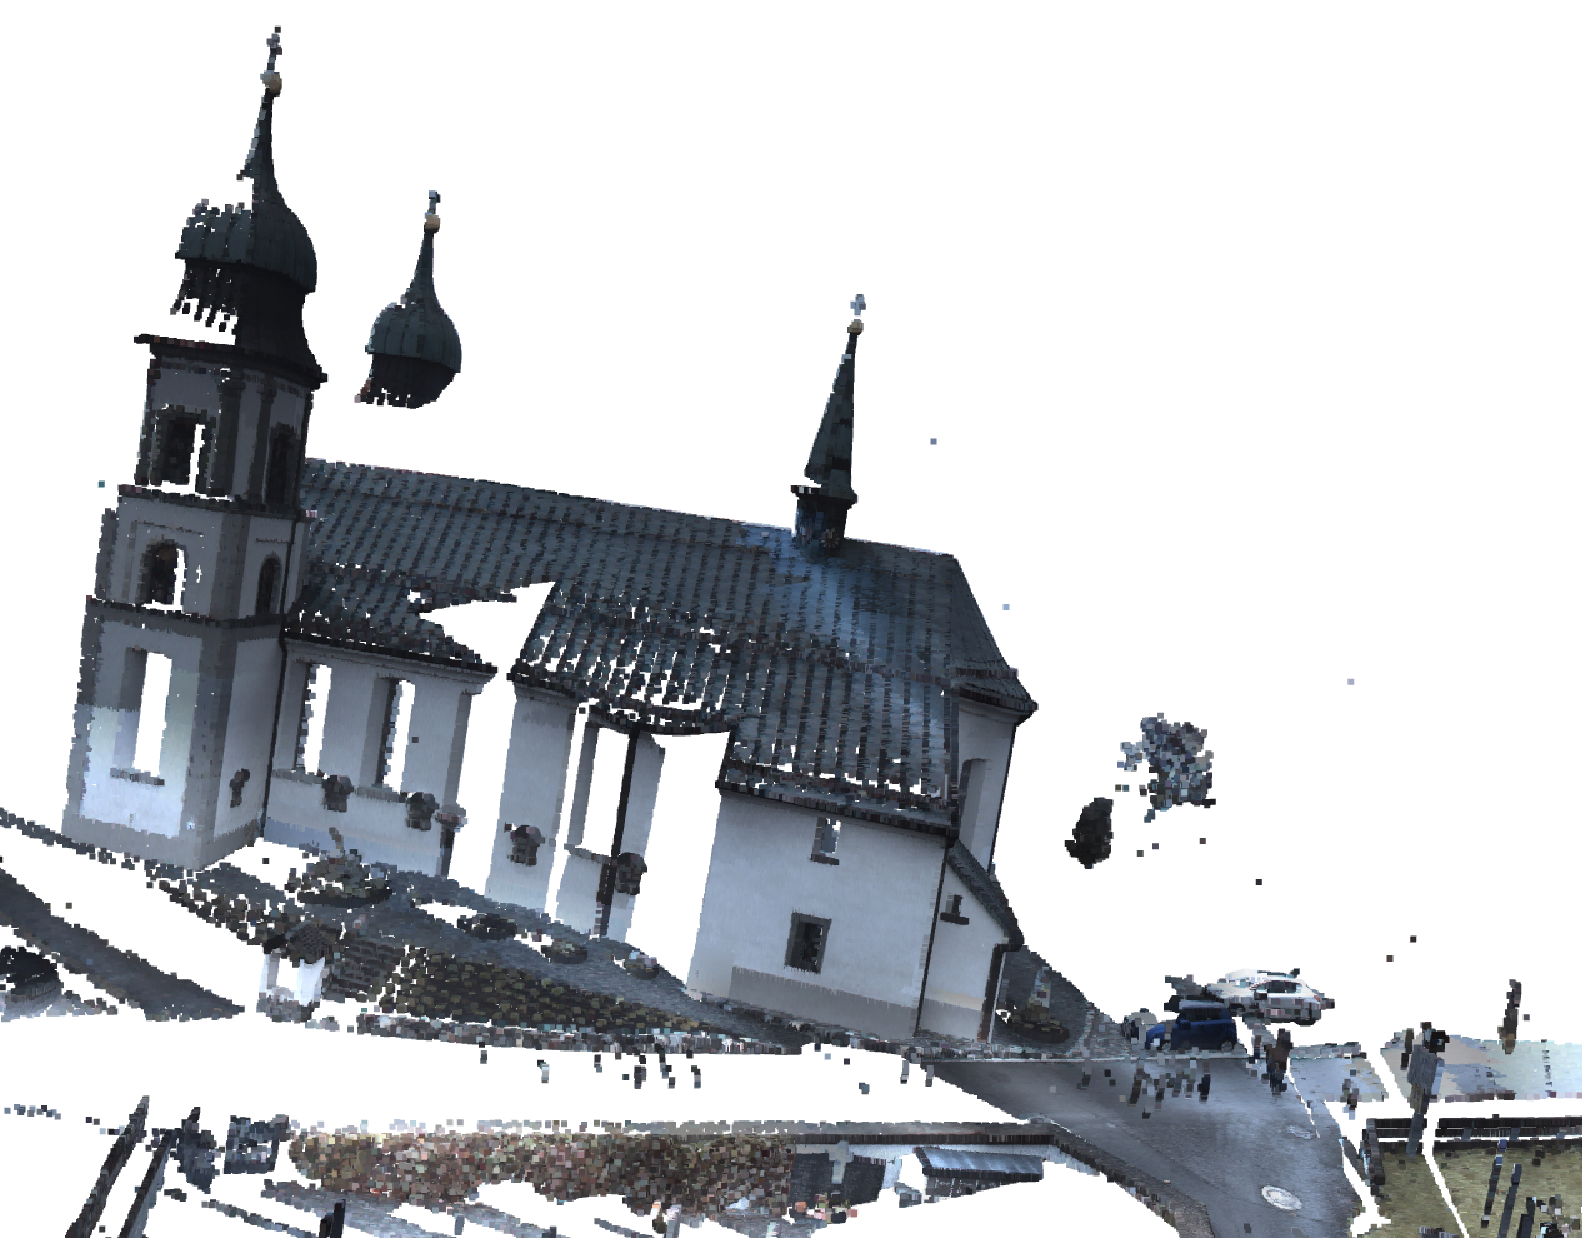
\includegraphics[width=0.35\textwidth, height=0.15\textheight]{images/sem3d_data/1.pdf} &
        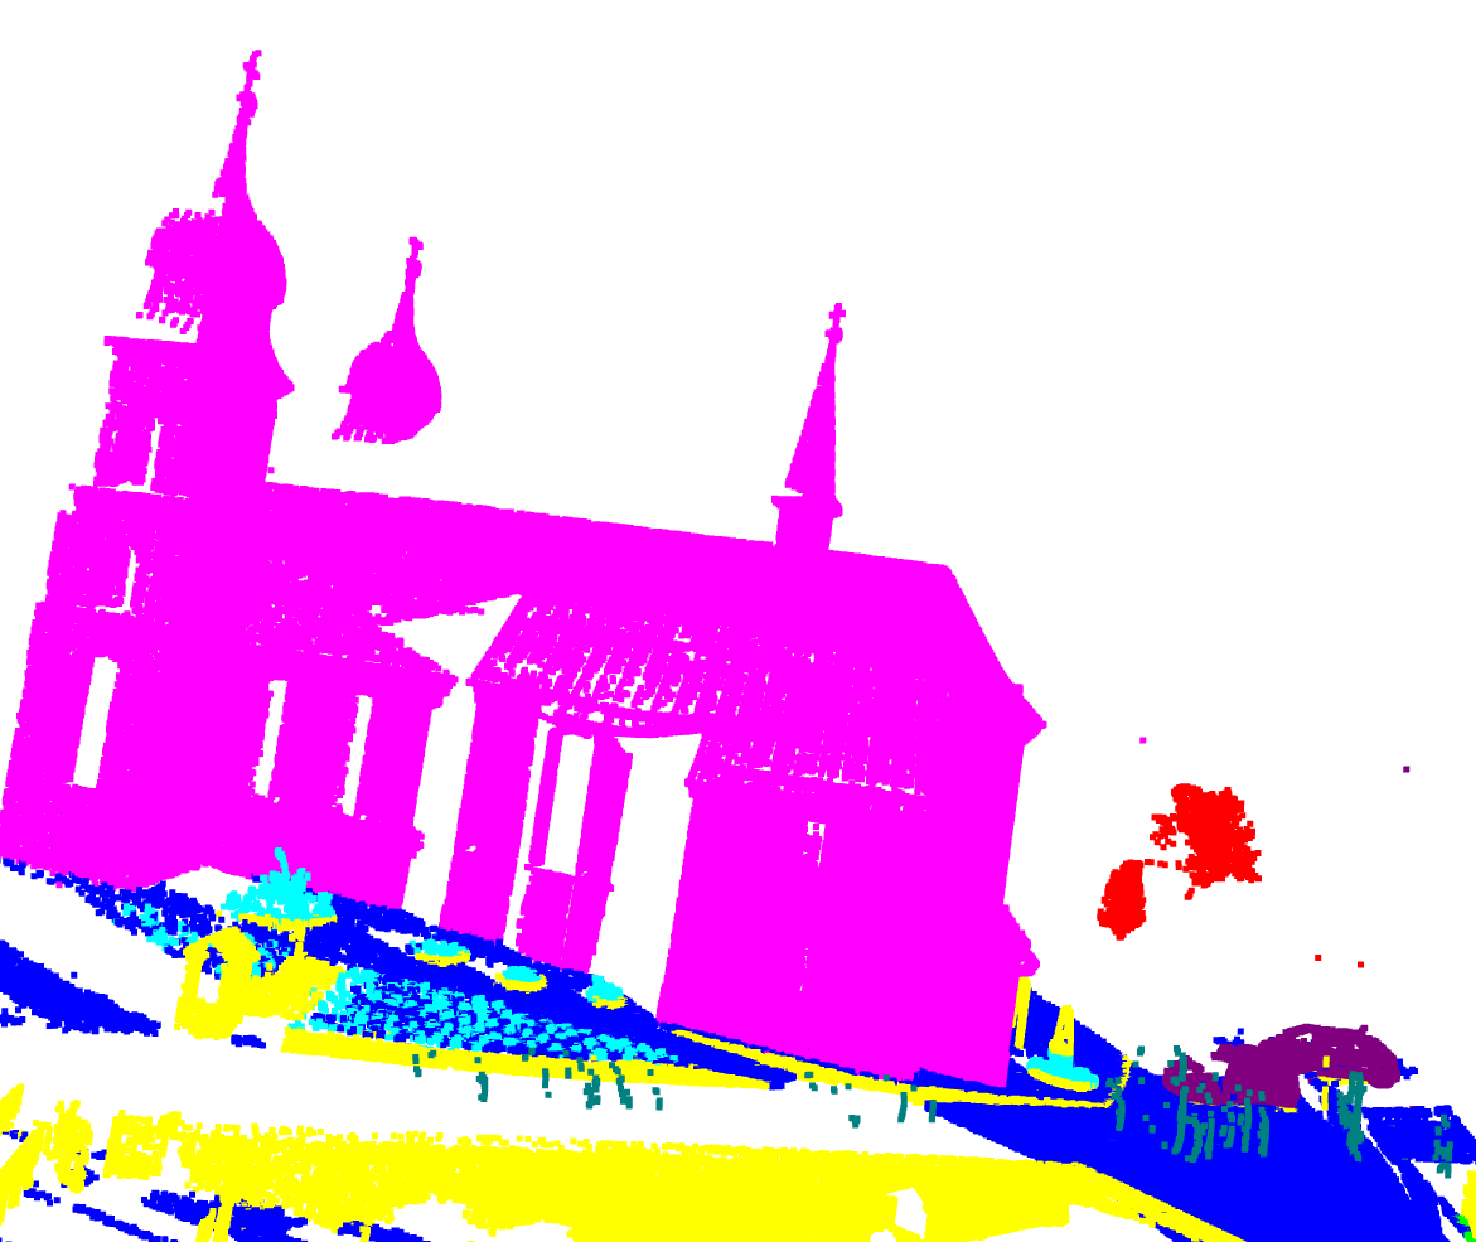
\includegraphics[width=0.35\textwidth, height=0.15\textheight]{images/sem3d_data/1_gt.pdf}\\
        
        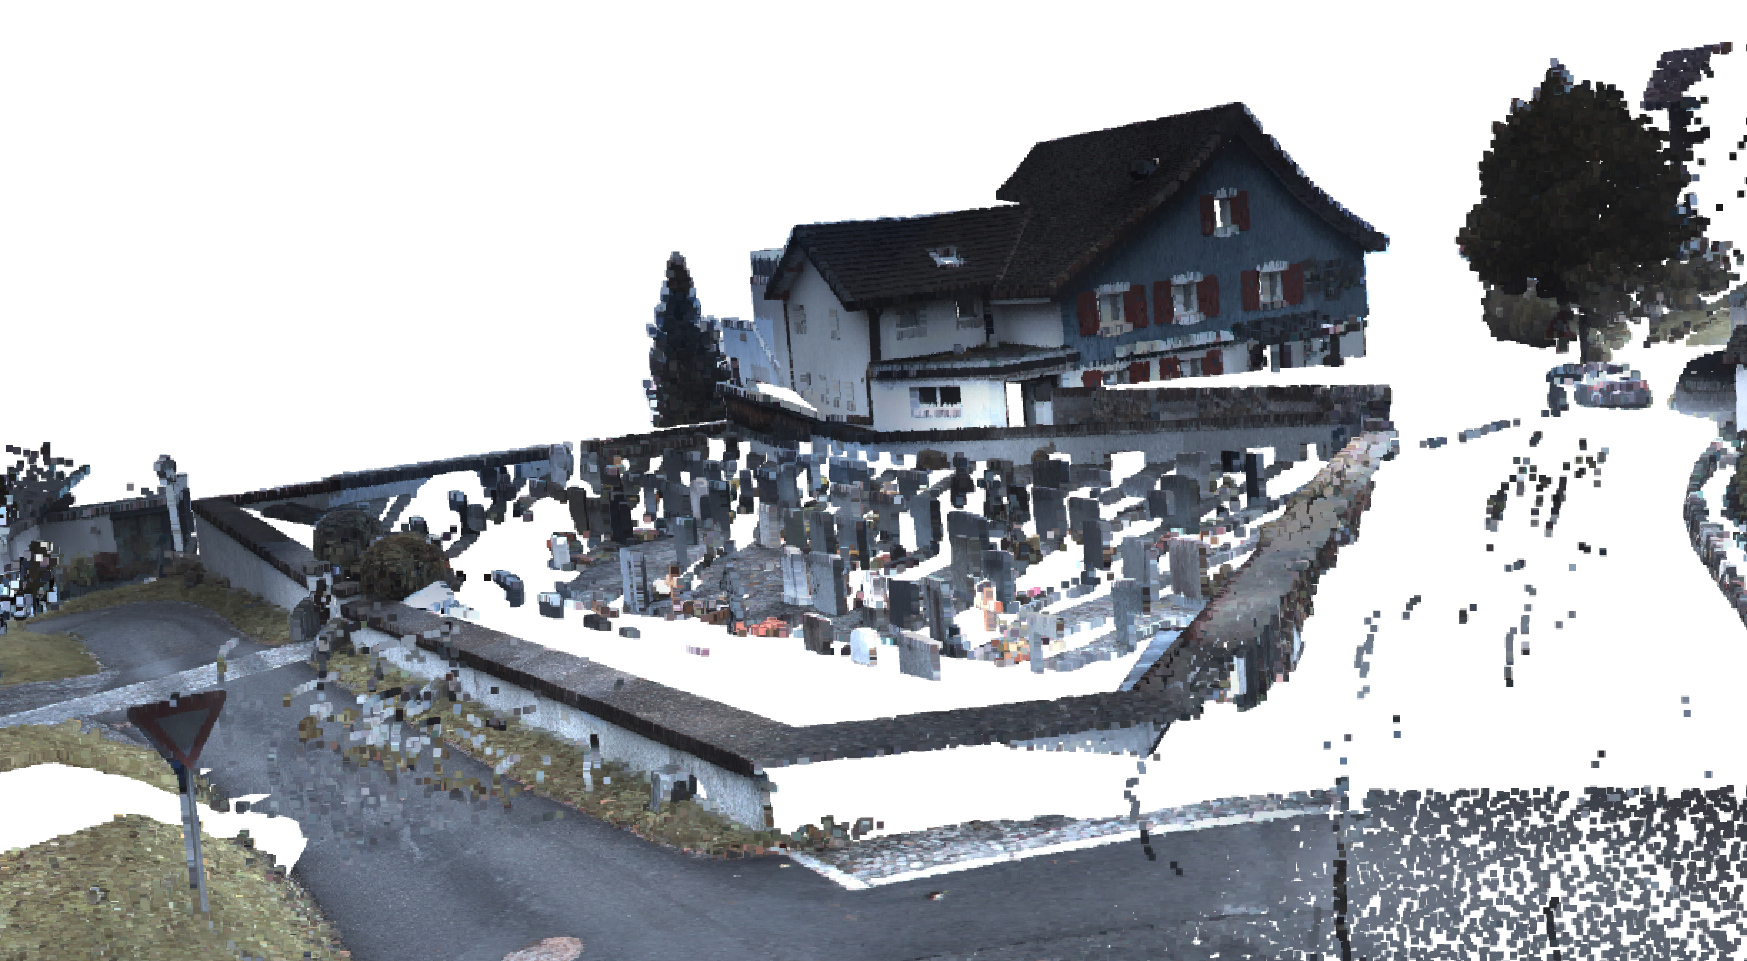
\includegraphics[width=0.35\textwidth, height=0.15\textheight]{images/sem3d_data/2.pdf} & 
        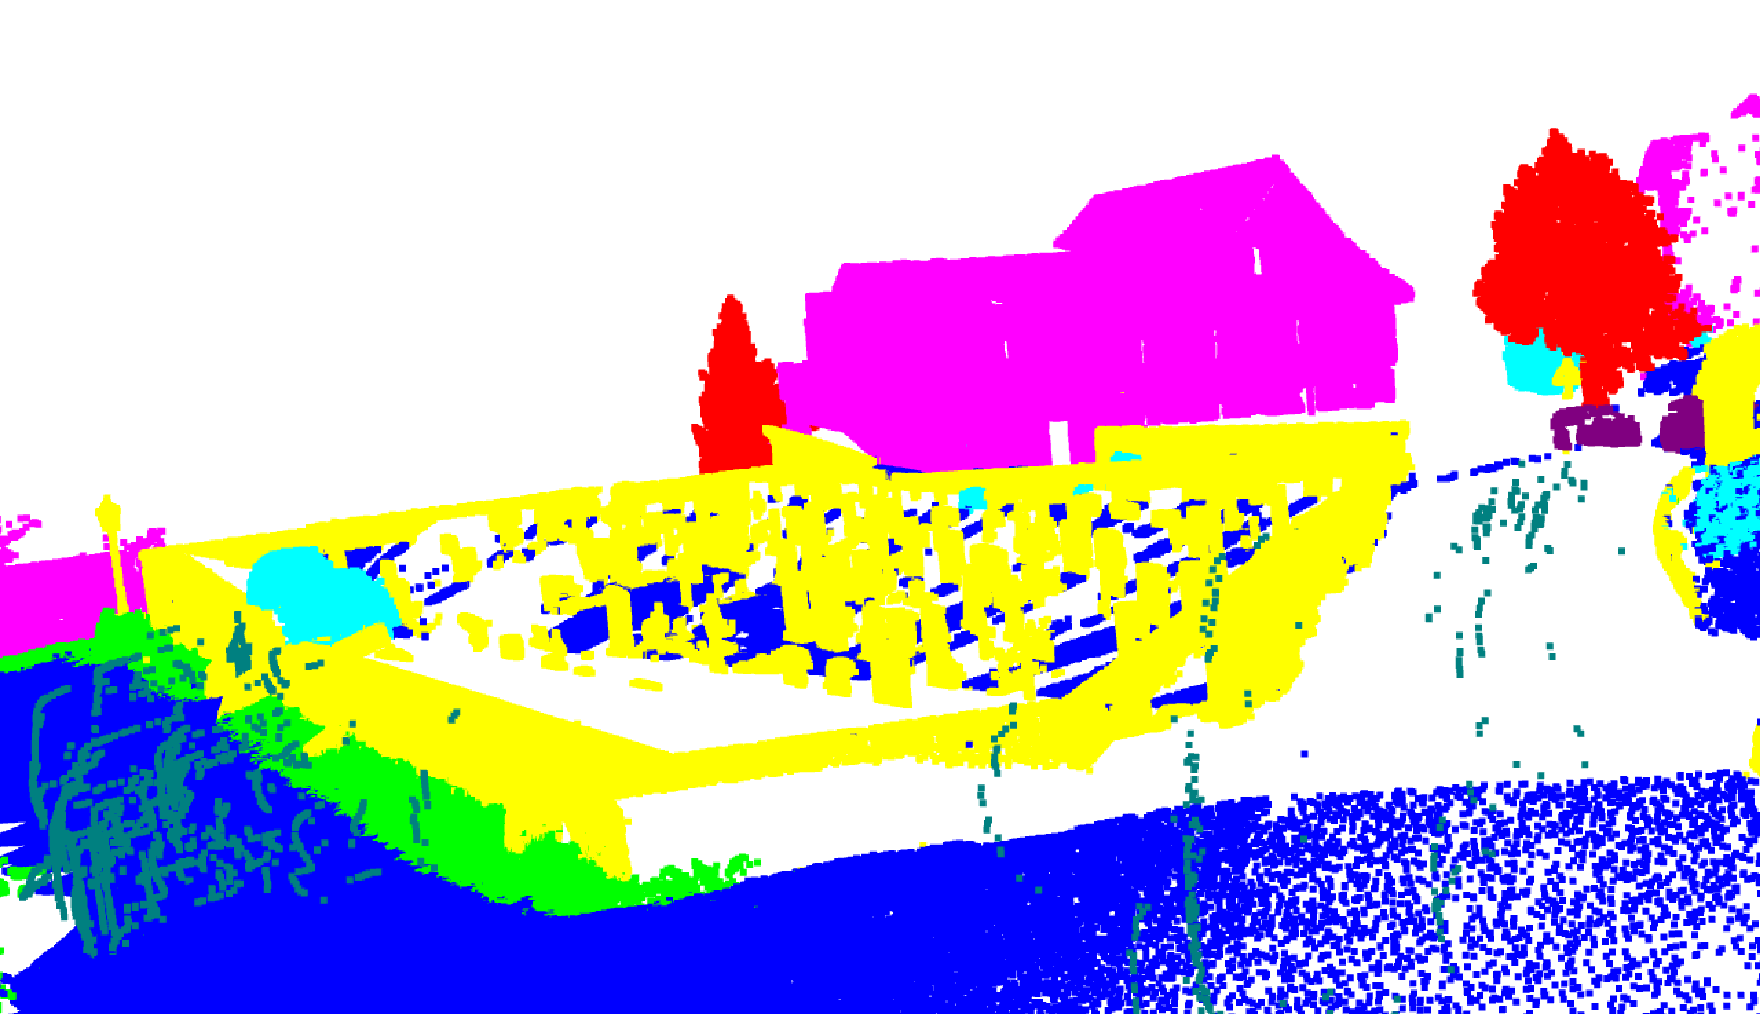
\includegraphics[width=0.35\textwidth, height=0.15\textheight]{images/sem3d_data/2_gt.pdf}\\
        
        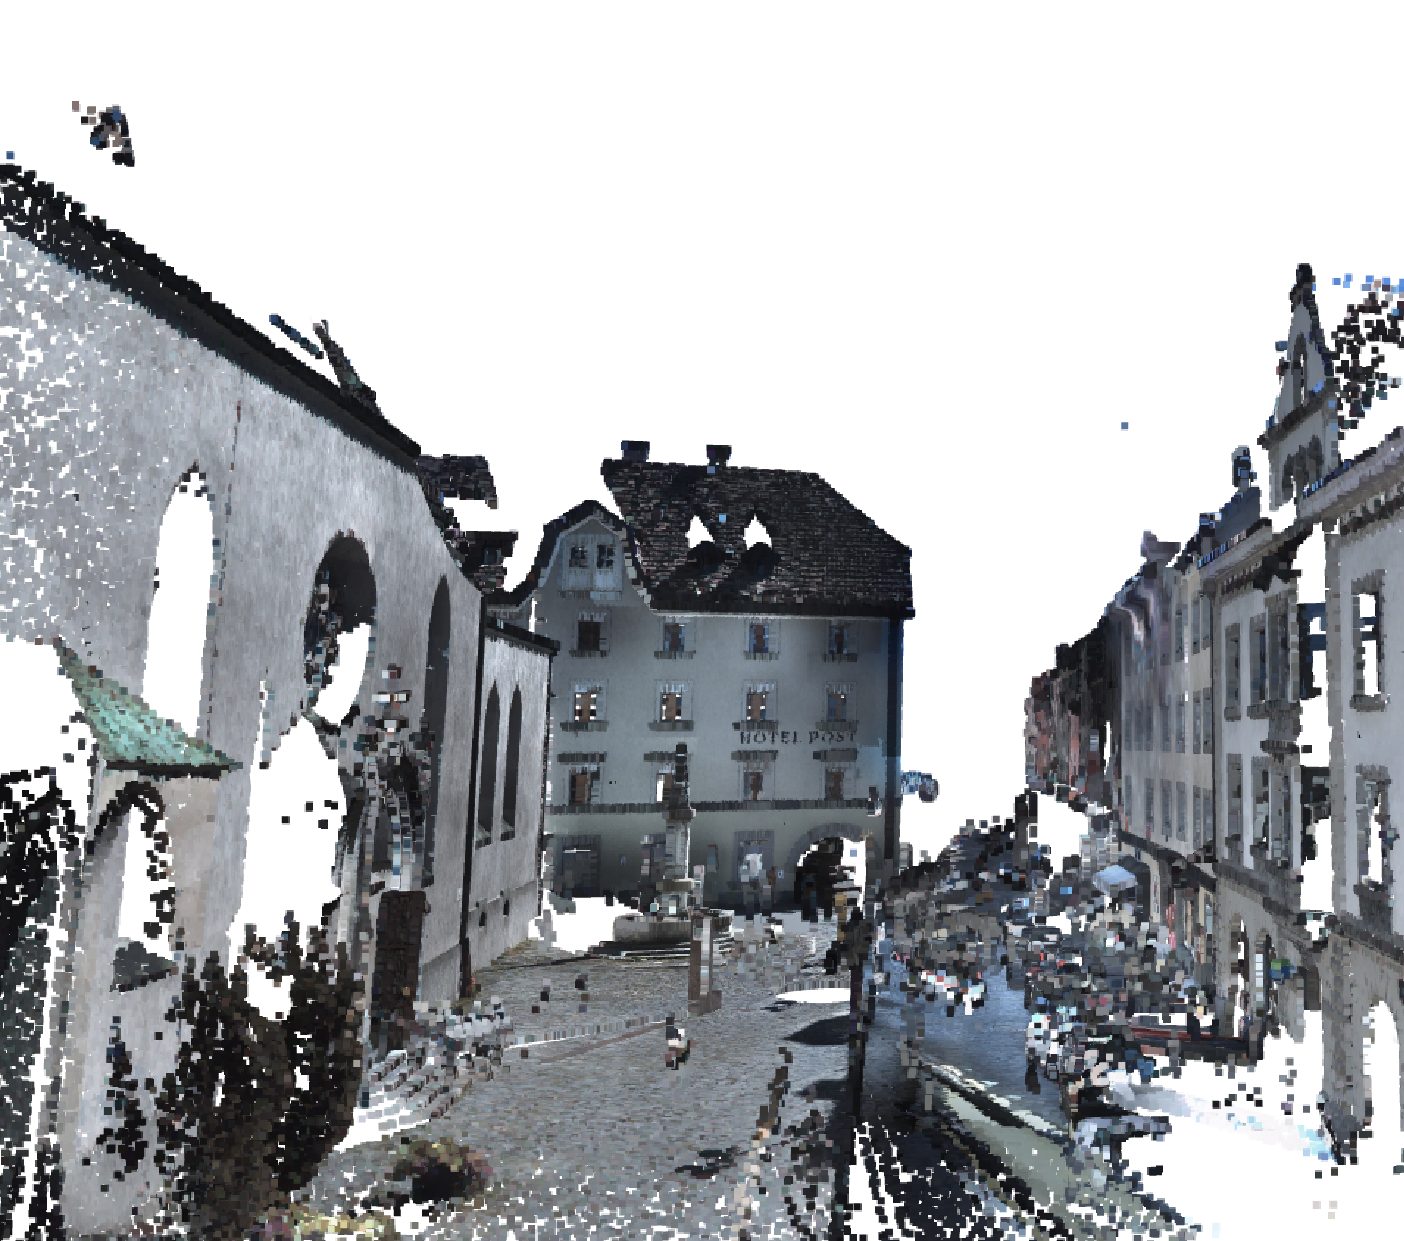
\includegraphics[width=0.35\textwidth, height=0.15\textheight]{images/sem3d_data/3.pdf} & 
        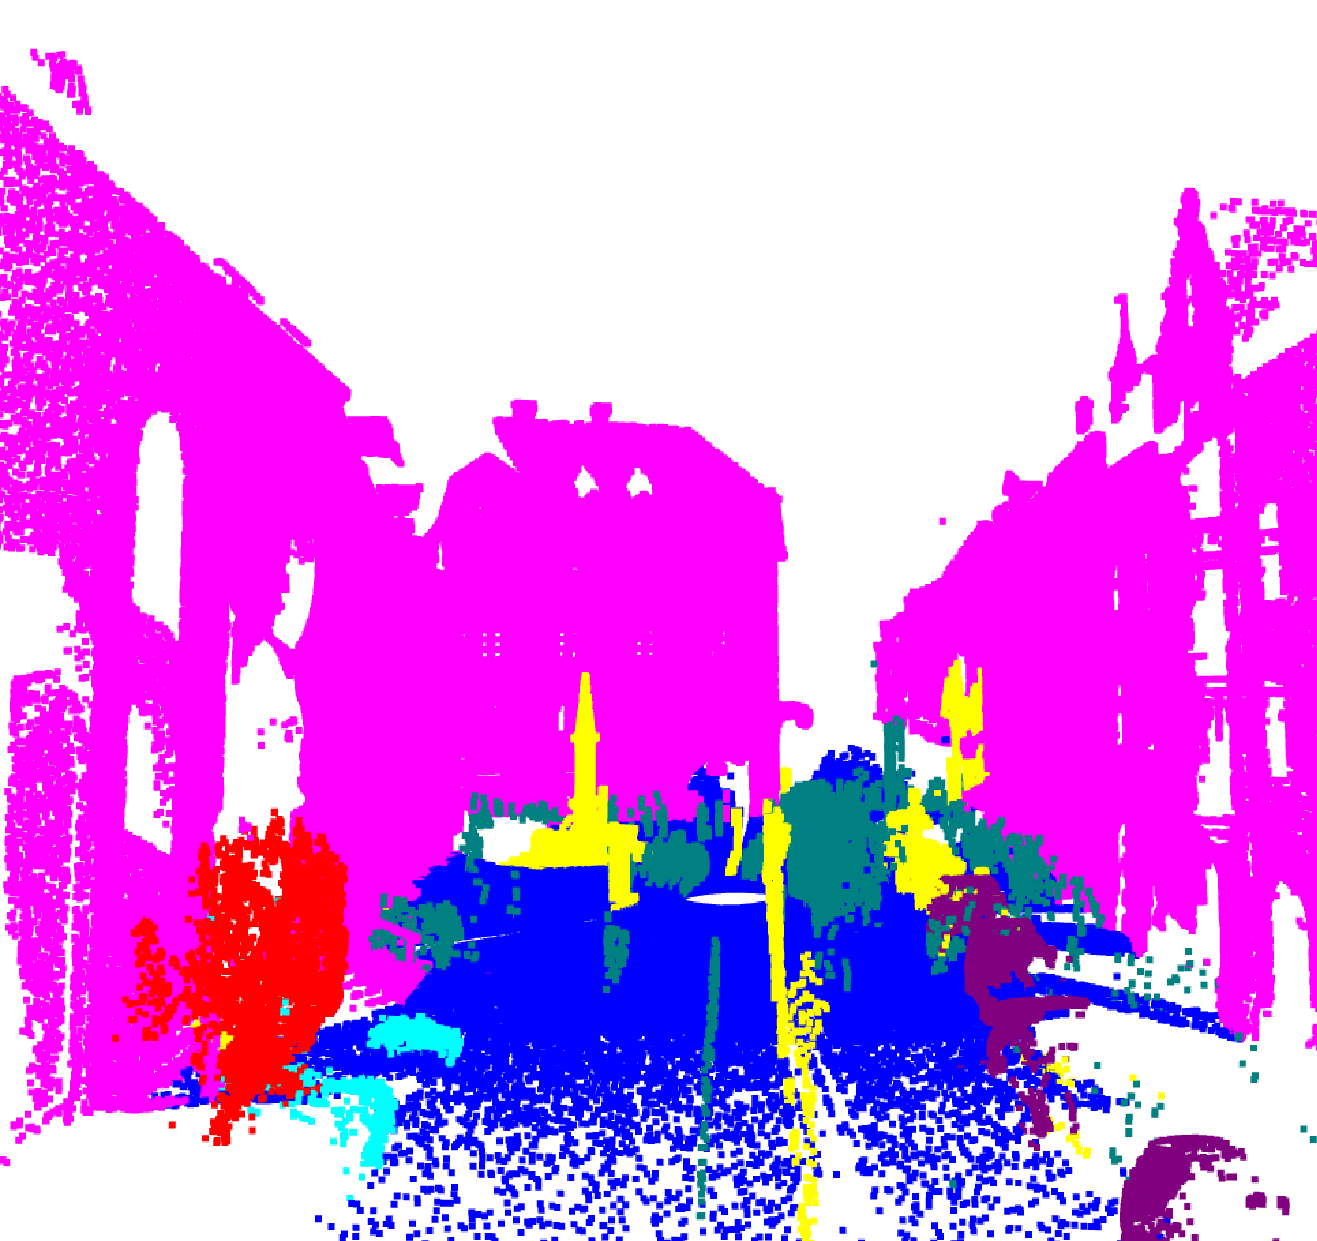
\includegraphics[width=0.35\textwidth, height=0.15\textheight]{images/sem3d_data/3_gt.pdf}\\
        
        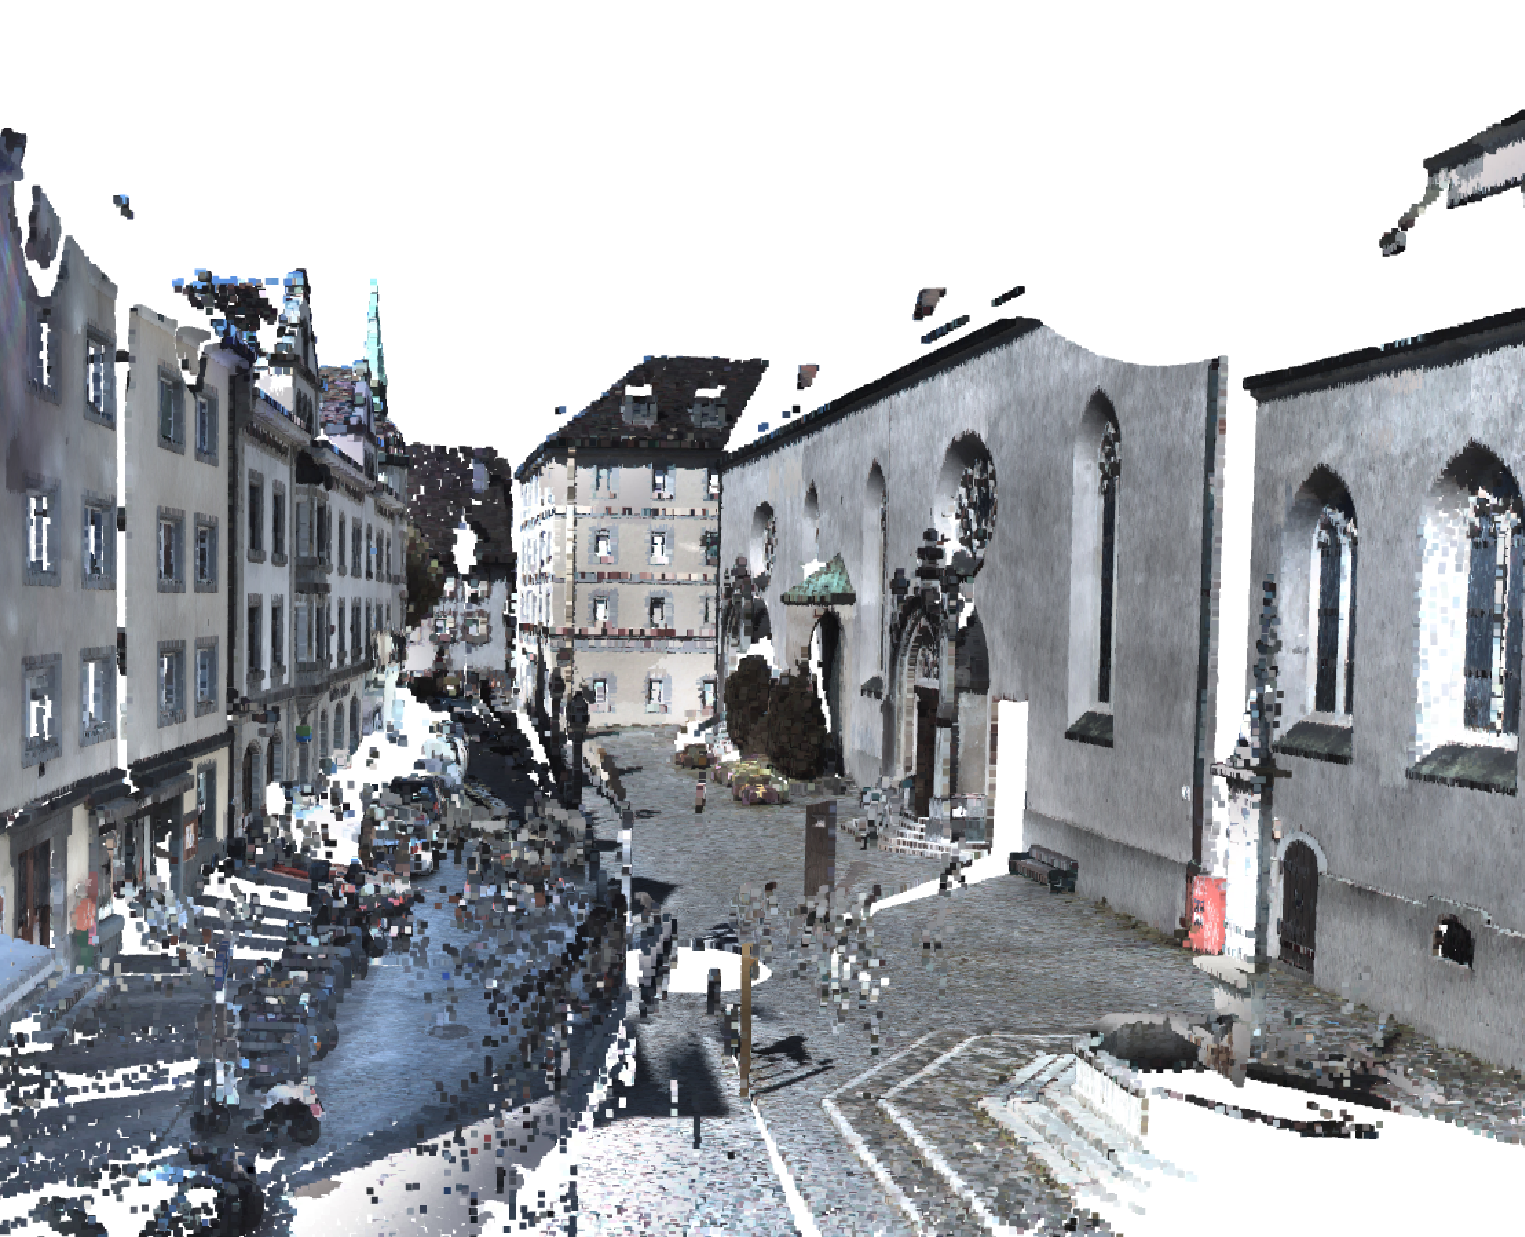
\includegraphics[width=0.35\textwidth, height=0.15\textheight]{images/sem3d_data/4.pdf} & 
        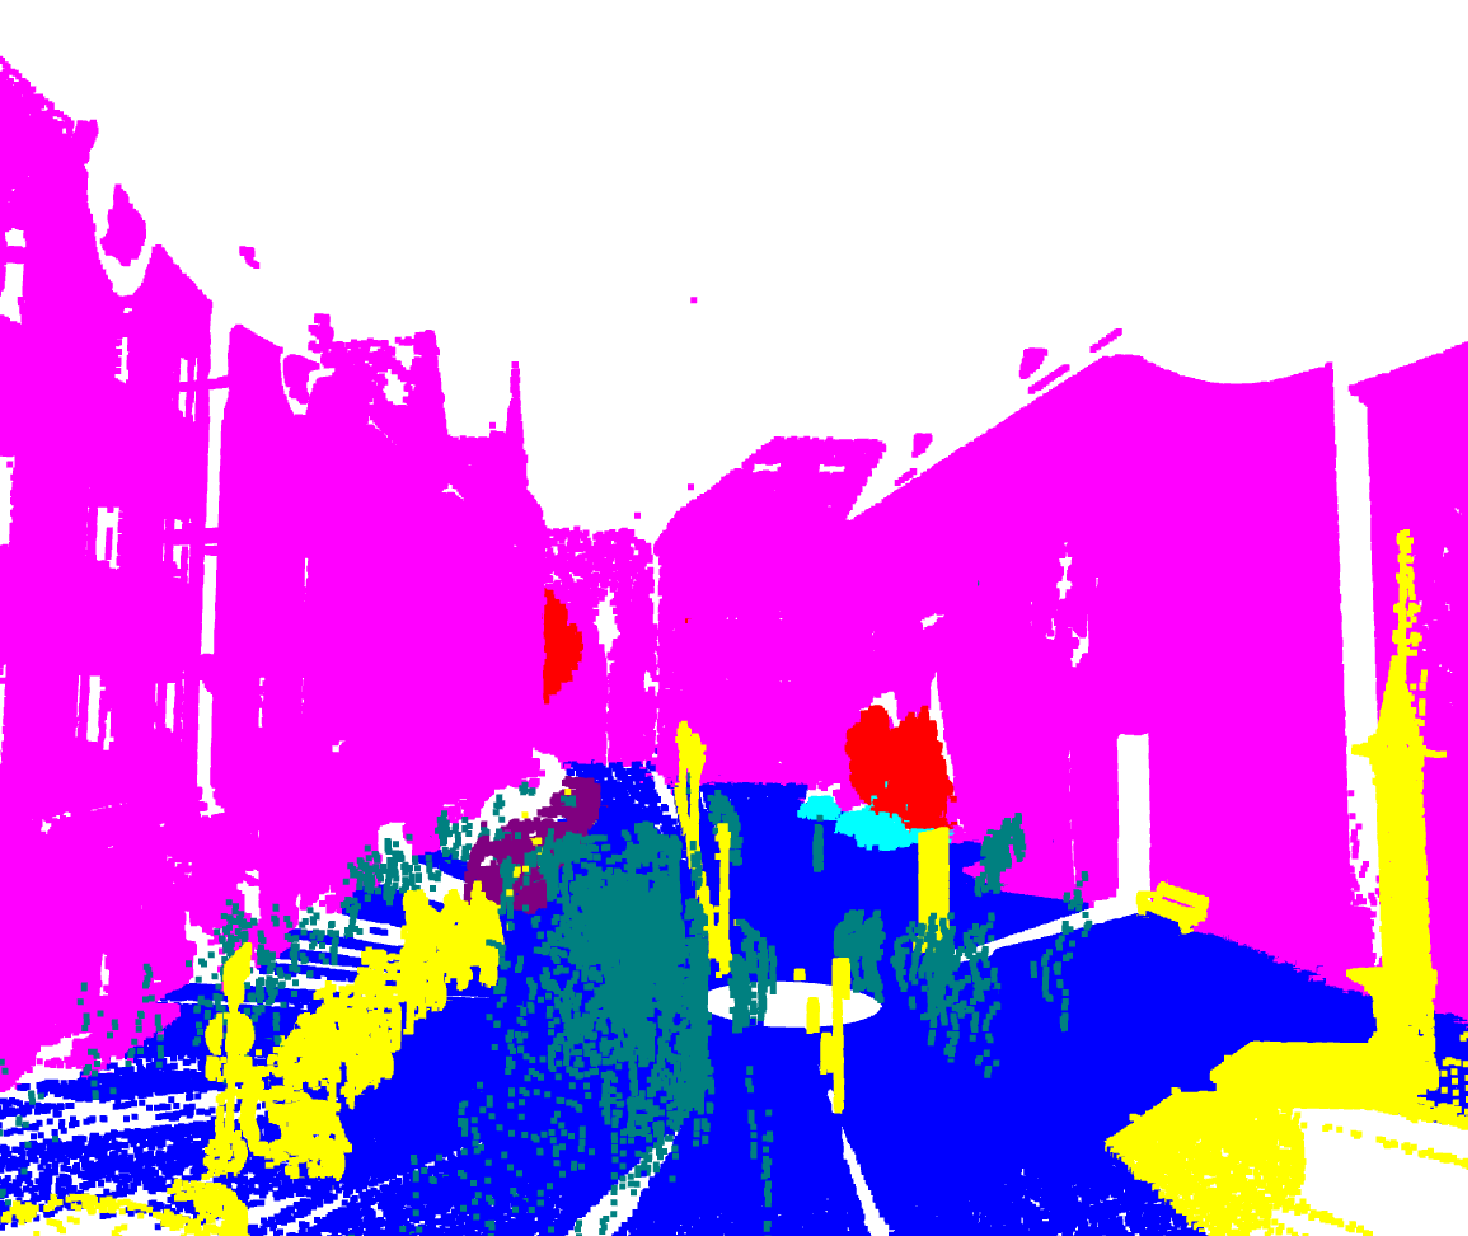
\includegraphics[width=0.35\textwidth, height=0.15\textheight]{images/sem3d_data/4_gt.pdf}\\
        
        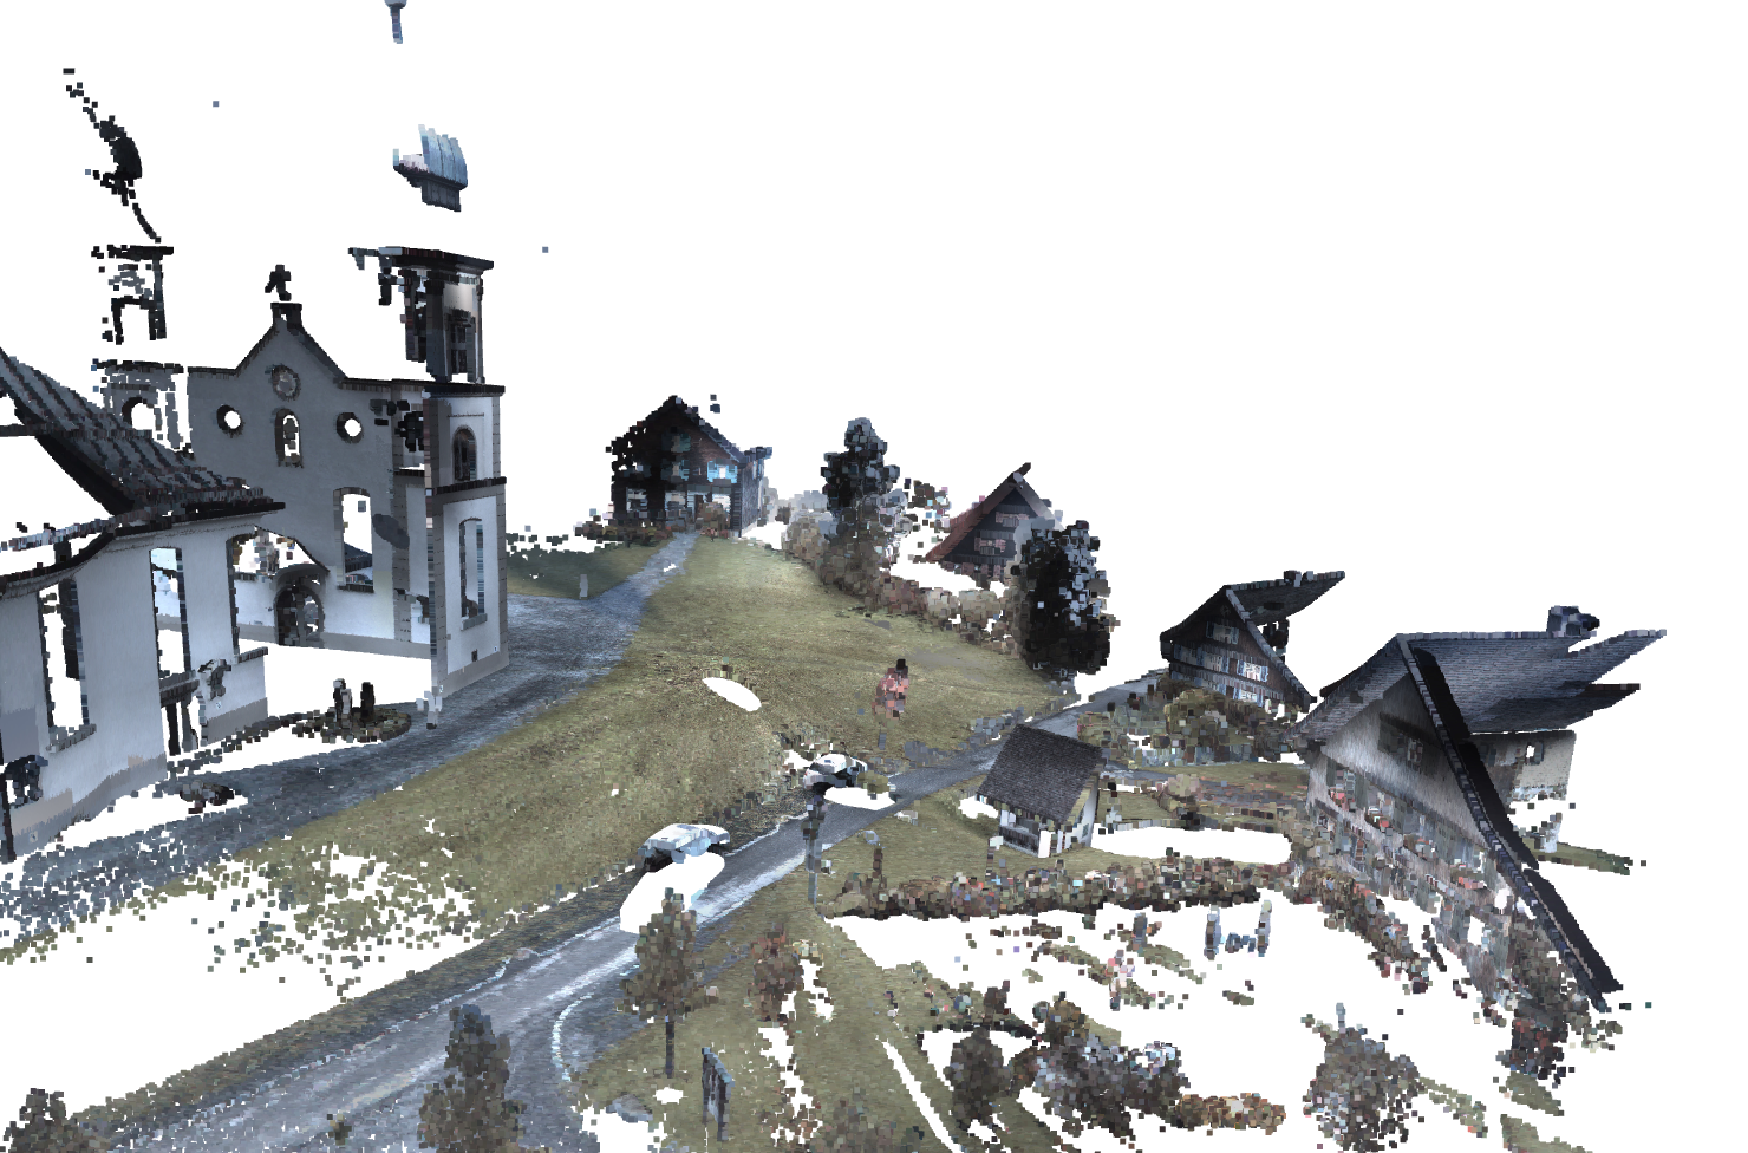
\includegraphics[width=0.35\textwidth, height=0.15\textheight]{images/sem3d_data/5.pdf} & 
        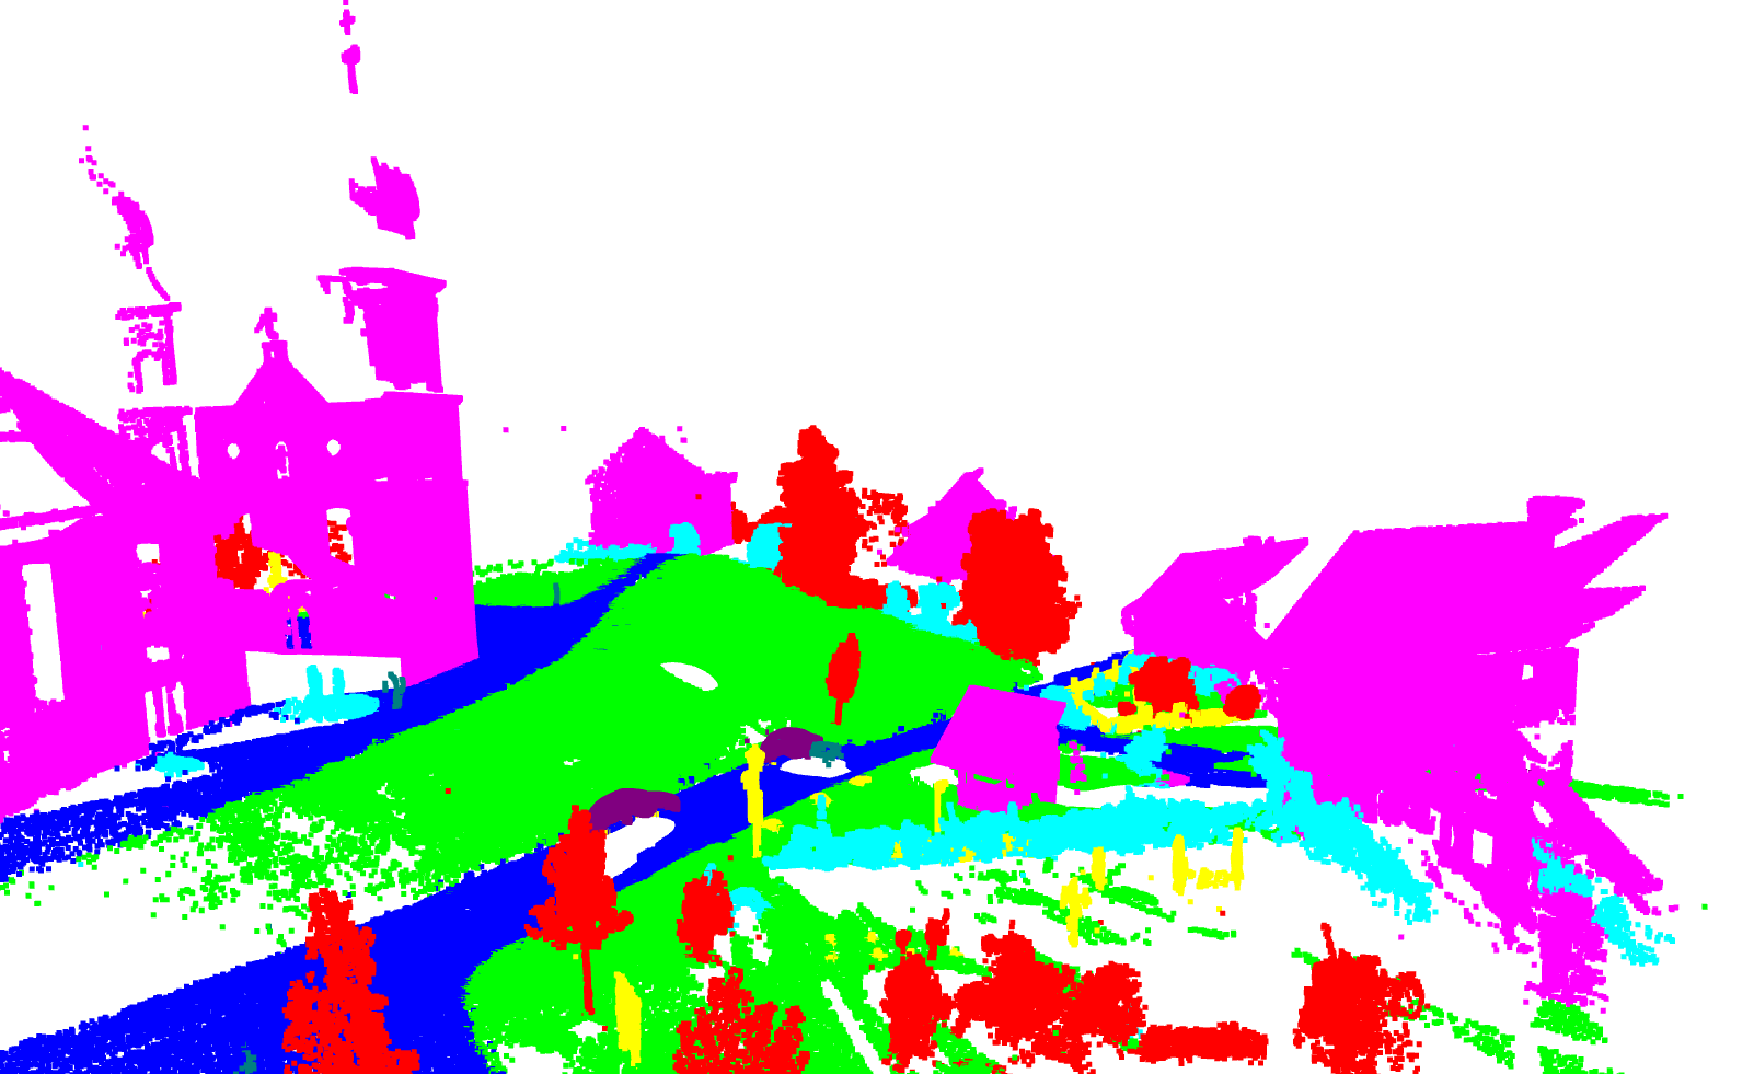
\includegraphics[width=0.35\textwidth, height=0.15\textheight]{images/sem3d_data/5_gt.pdf}\\
    \end{tabular}
    
\includegraphics[scale=0.45]{images/legend.png}
    \caption{Illustration of the Semantic3D point clouds in training and validation set with first column representing the point cloud 
    and second column their repective ground truth with legend for ground truth given in last image.}
    \label{fig:sem3d_gt_vis}
\end{figure*}

\section{S3DIS}
\label{sec:dataset_s3dis}
S3DIS is an indoor dataset making it an ideal OOD dataset candidate because of the no class overlap with the Semantic3D dataset.
It is only one of two datasets available in indoor LiDAR dataset candidates. 
The other is ScanObjectNN, whose dataset is not available online.
S3DIS dataset comprises scans of three different buildings covering 6020 square meters.
These scans include personal offices, restrooms, open spaces, lobbies and hallways.
The scans are generated using Matterport 3D scanner as a triangular mesh and can be seen in Figure~\ref{fig:how_matterport_works}.
S3DIS dataset is divided into 12 classes, further divided into two subclasses.
The first subclass includes structural elements, which consist of \textit{ceiling, floor, window, wall, beam, columns and door}
Furthermore, the latter subclass has everyday items such as \textit{table, sofa, chair, board and blackboard}.
Along with ShapeNet dataset \cite{chang2015shapenet}, S3DIS is also one of the most evaluated dataset in indoor setting for semantic segmentation  using in \cite{Armeni_2016_CVPR_S3DIS} whereas ShapeNet is used for part segmentation.
\begin{figure}[!ht]
    \centering
    \begin{tabular}{cc}
        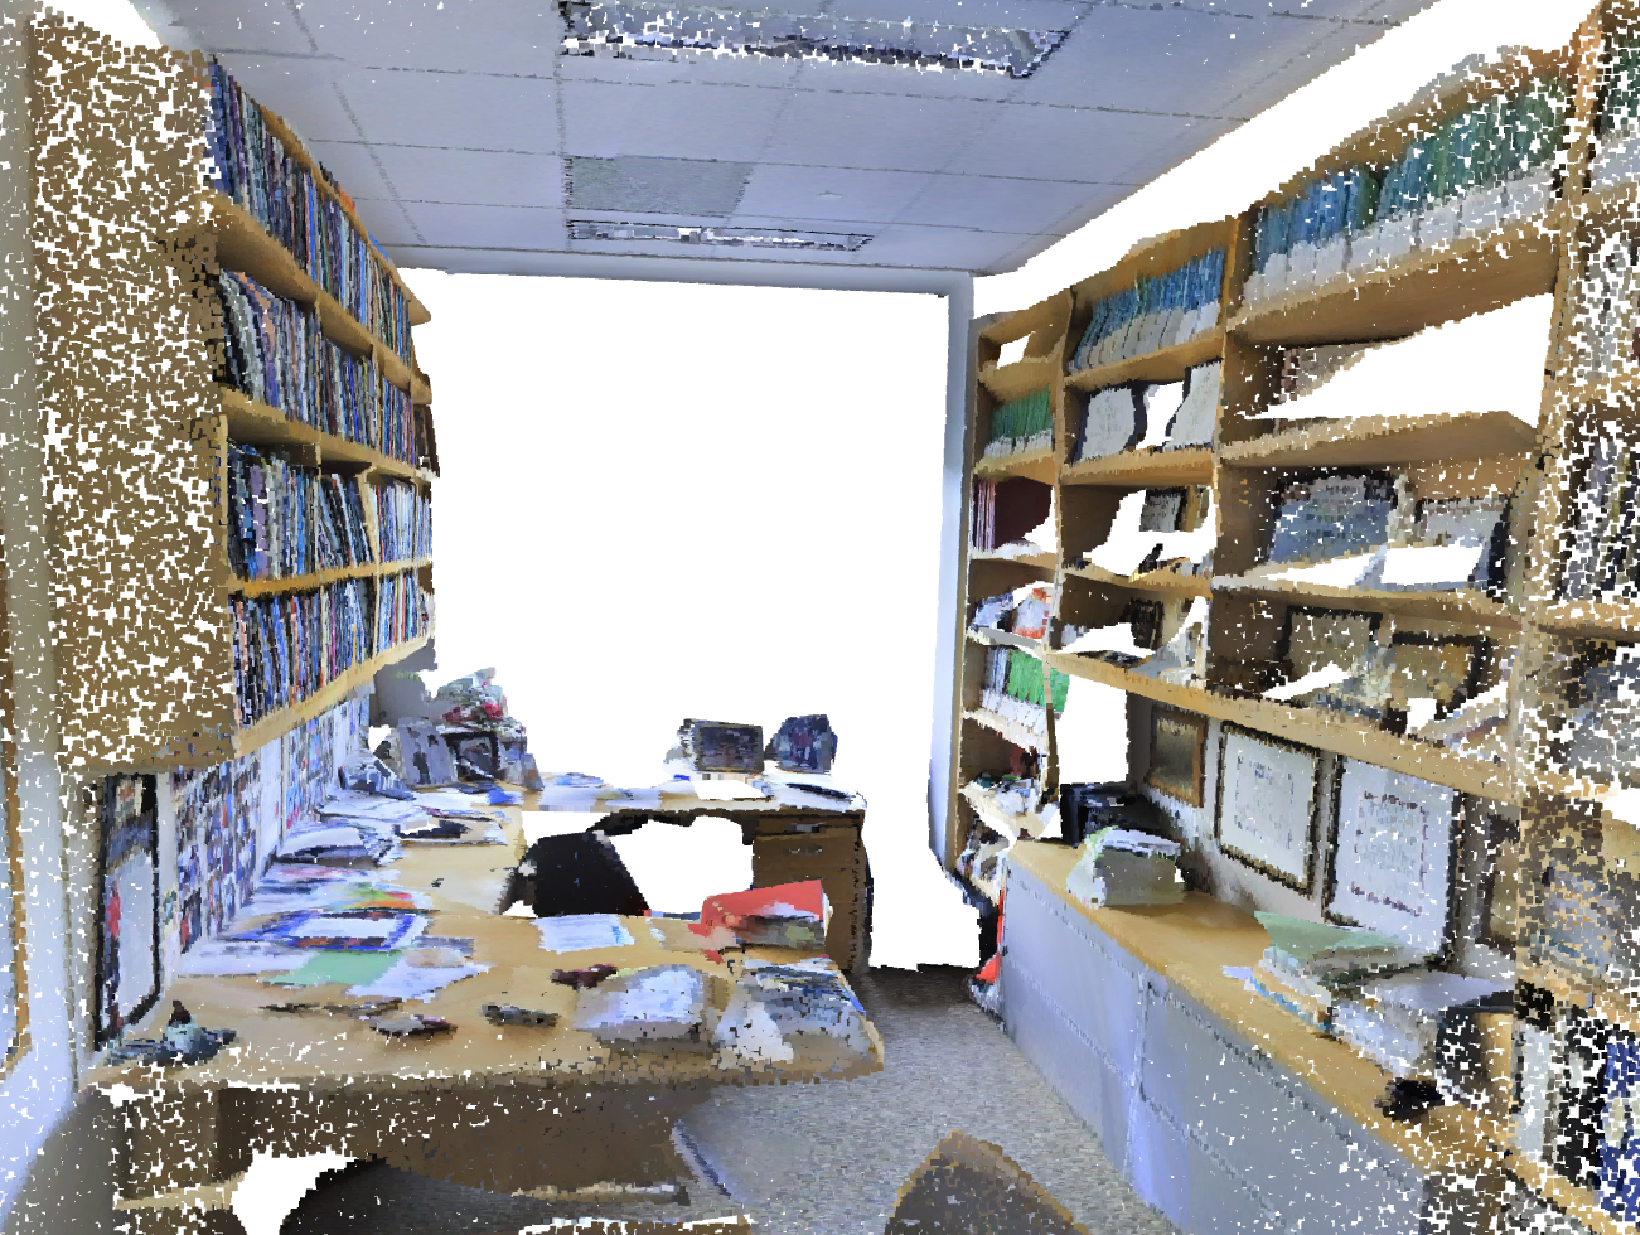
\includegraphics[width=0.35\textwidth, height=0.15\textheight]{images/seg_output/s3dis_DE/S3DIS_1_RGB.pdf} &
        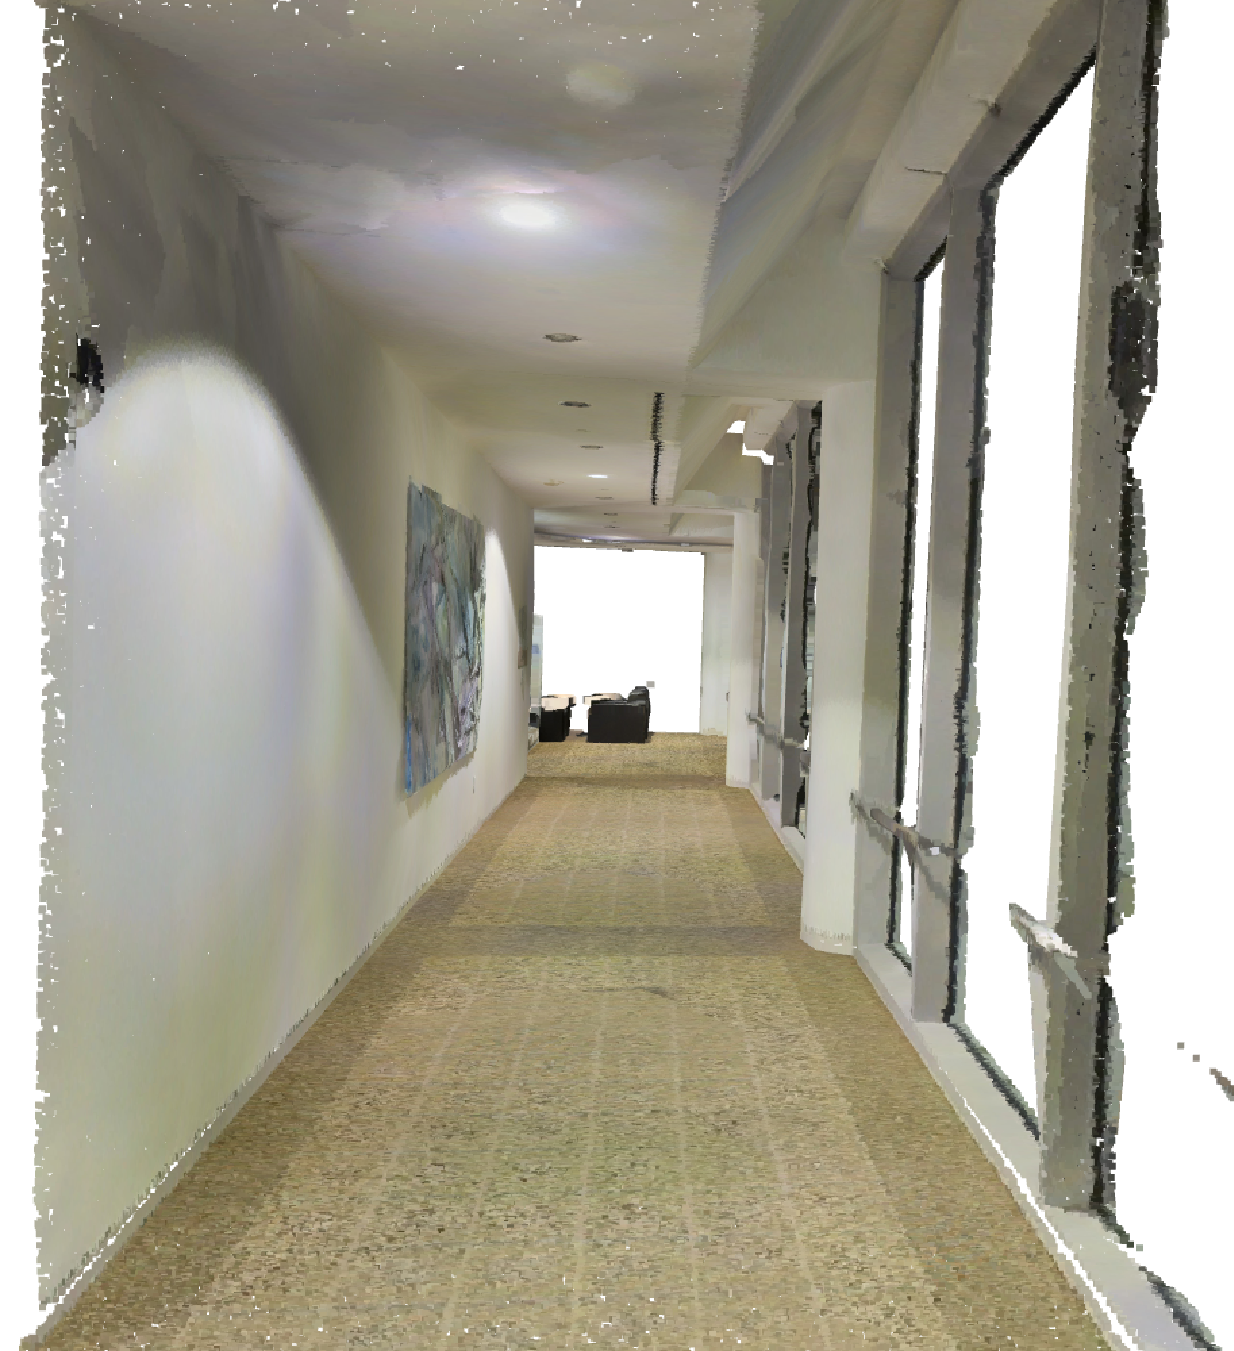
\includegraphics[width=0.35\textwidth, height=0.15\textheight]{images/seg_output/s3dis_DE/S3DIS_5_RGB.pdf} \\
        
        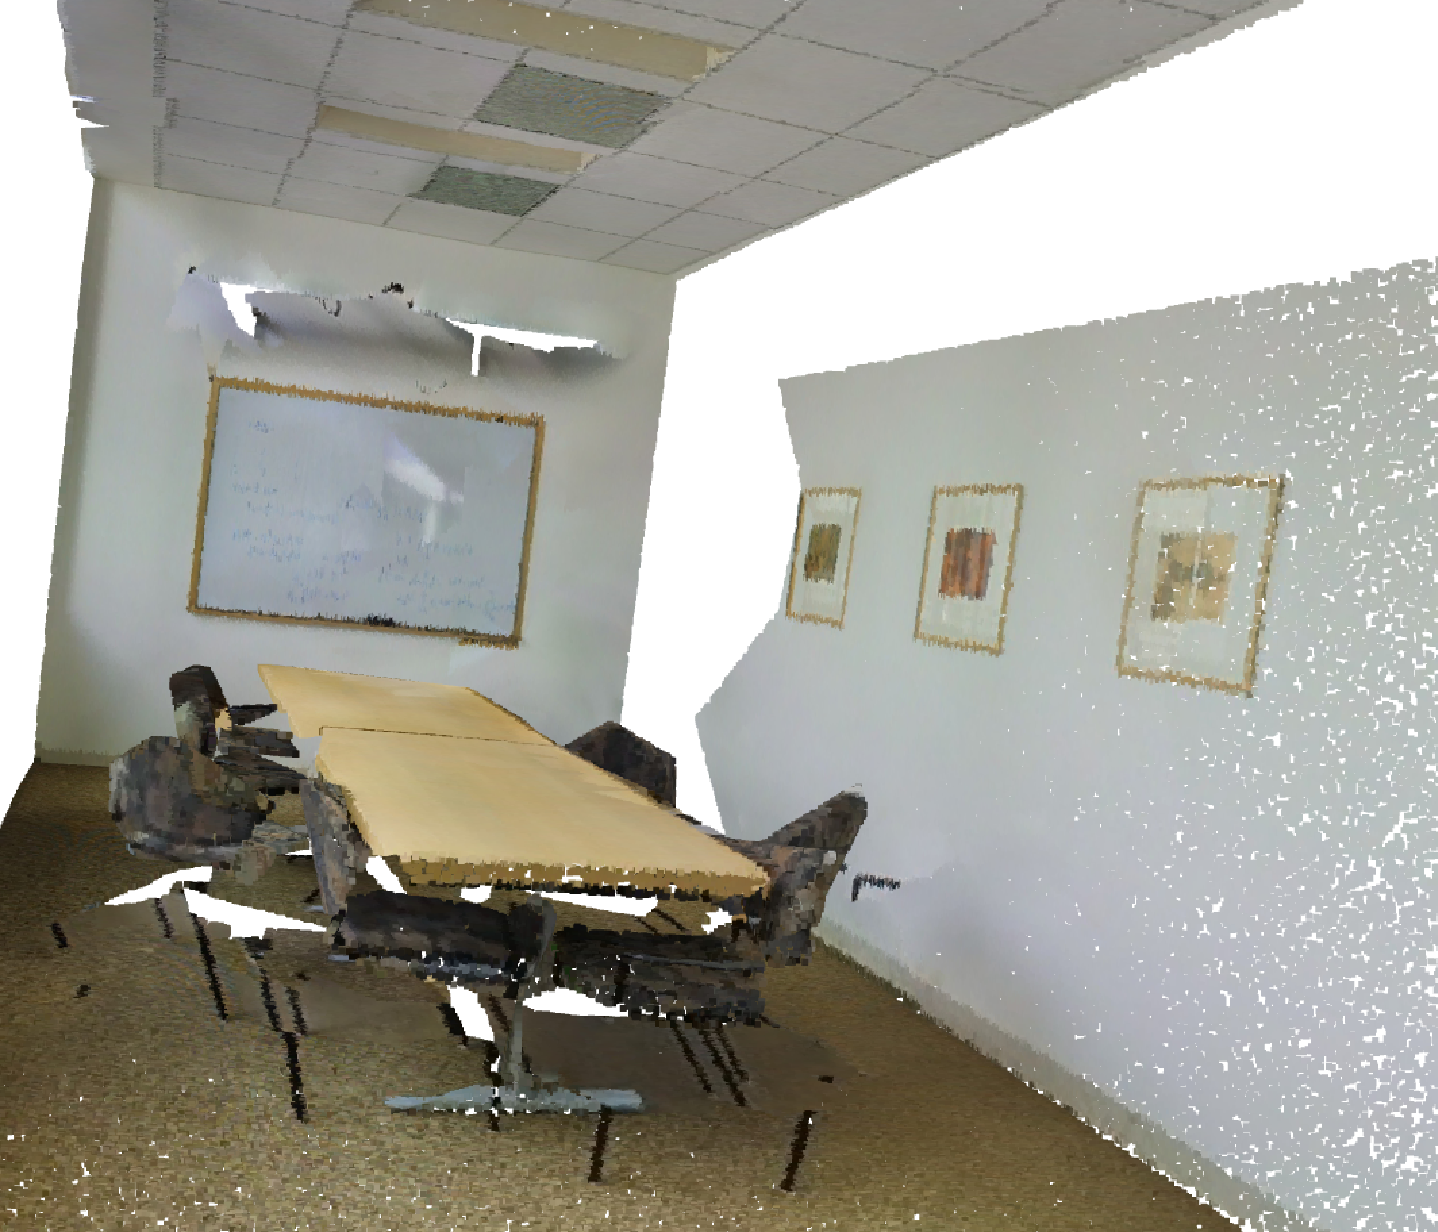
\includegraphics[width=0.35\textwidth, height=0.15\textheight]{images/seg_output/s3dis_DE/S3DIS_2_RGB.pdf} &
        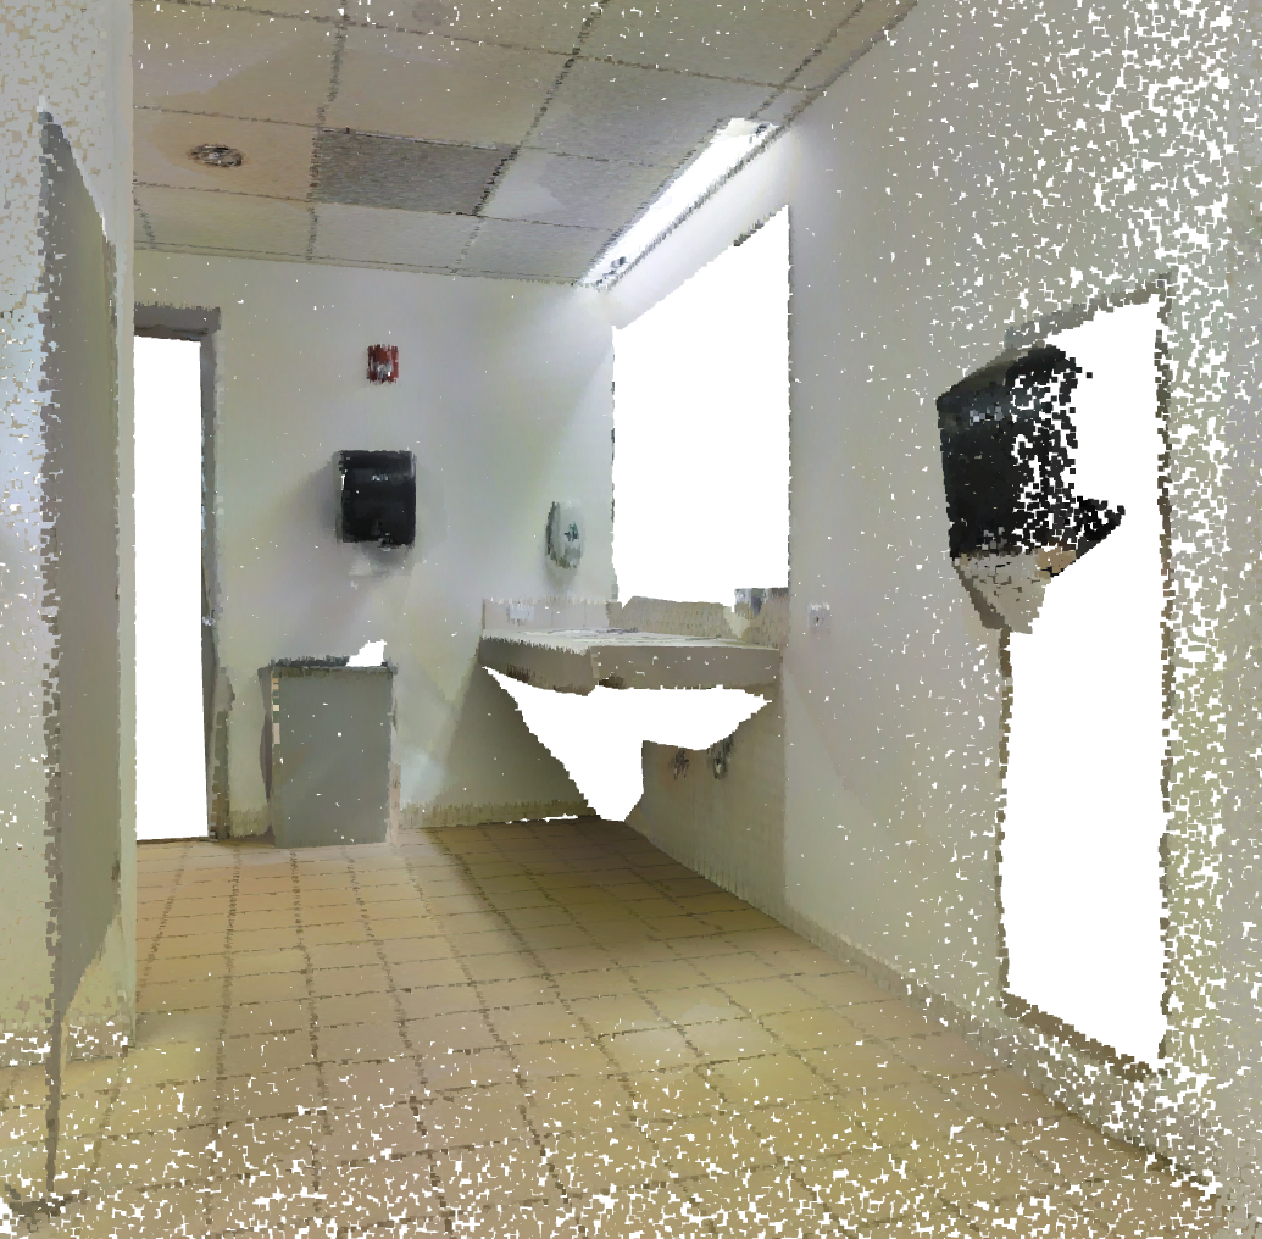
\includegraphics[width=0.35\textwidth, height=0.15\textheight]{images/seg_output/s3dis_DE/S3DIS_6_RGB.pdf} \\

        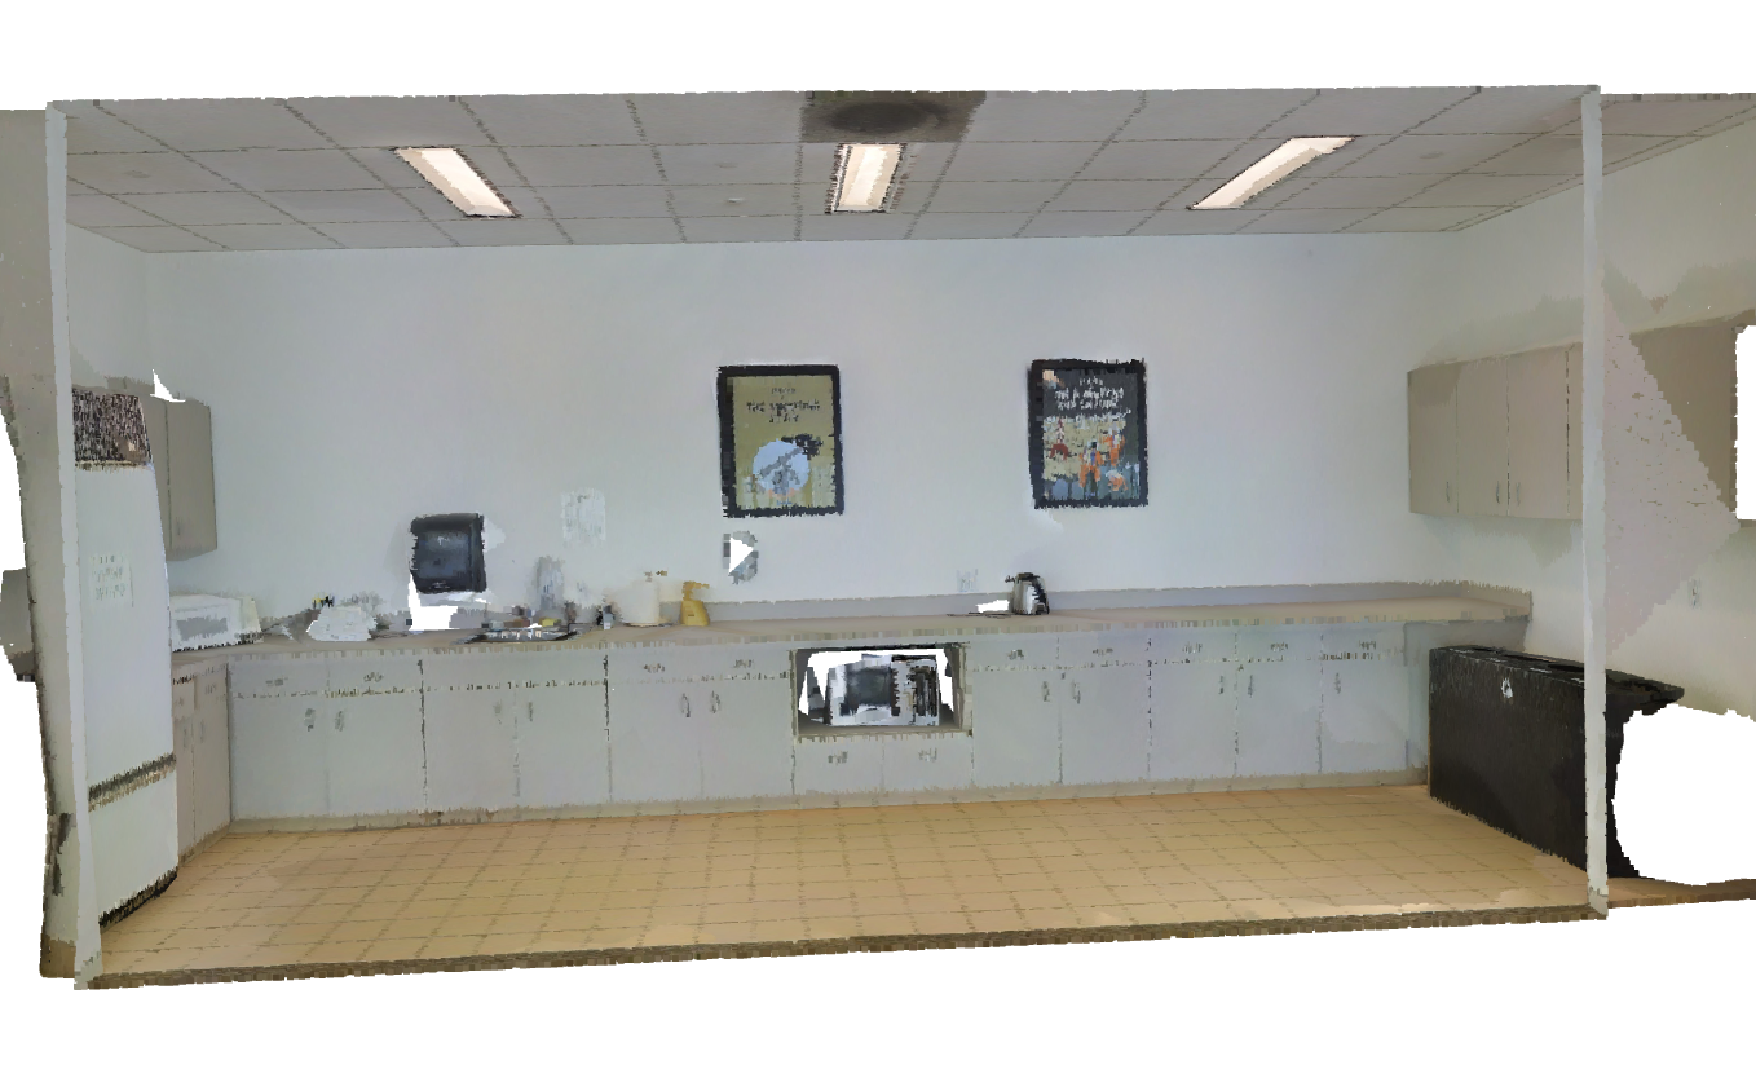
\includegraphics[width=0.35\textwidth, height=0.15\textheight]{images/seg_output/s3dis_DE/S3DIS_3_RGB.pdf} &
        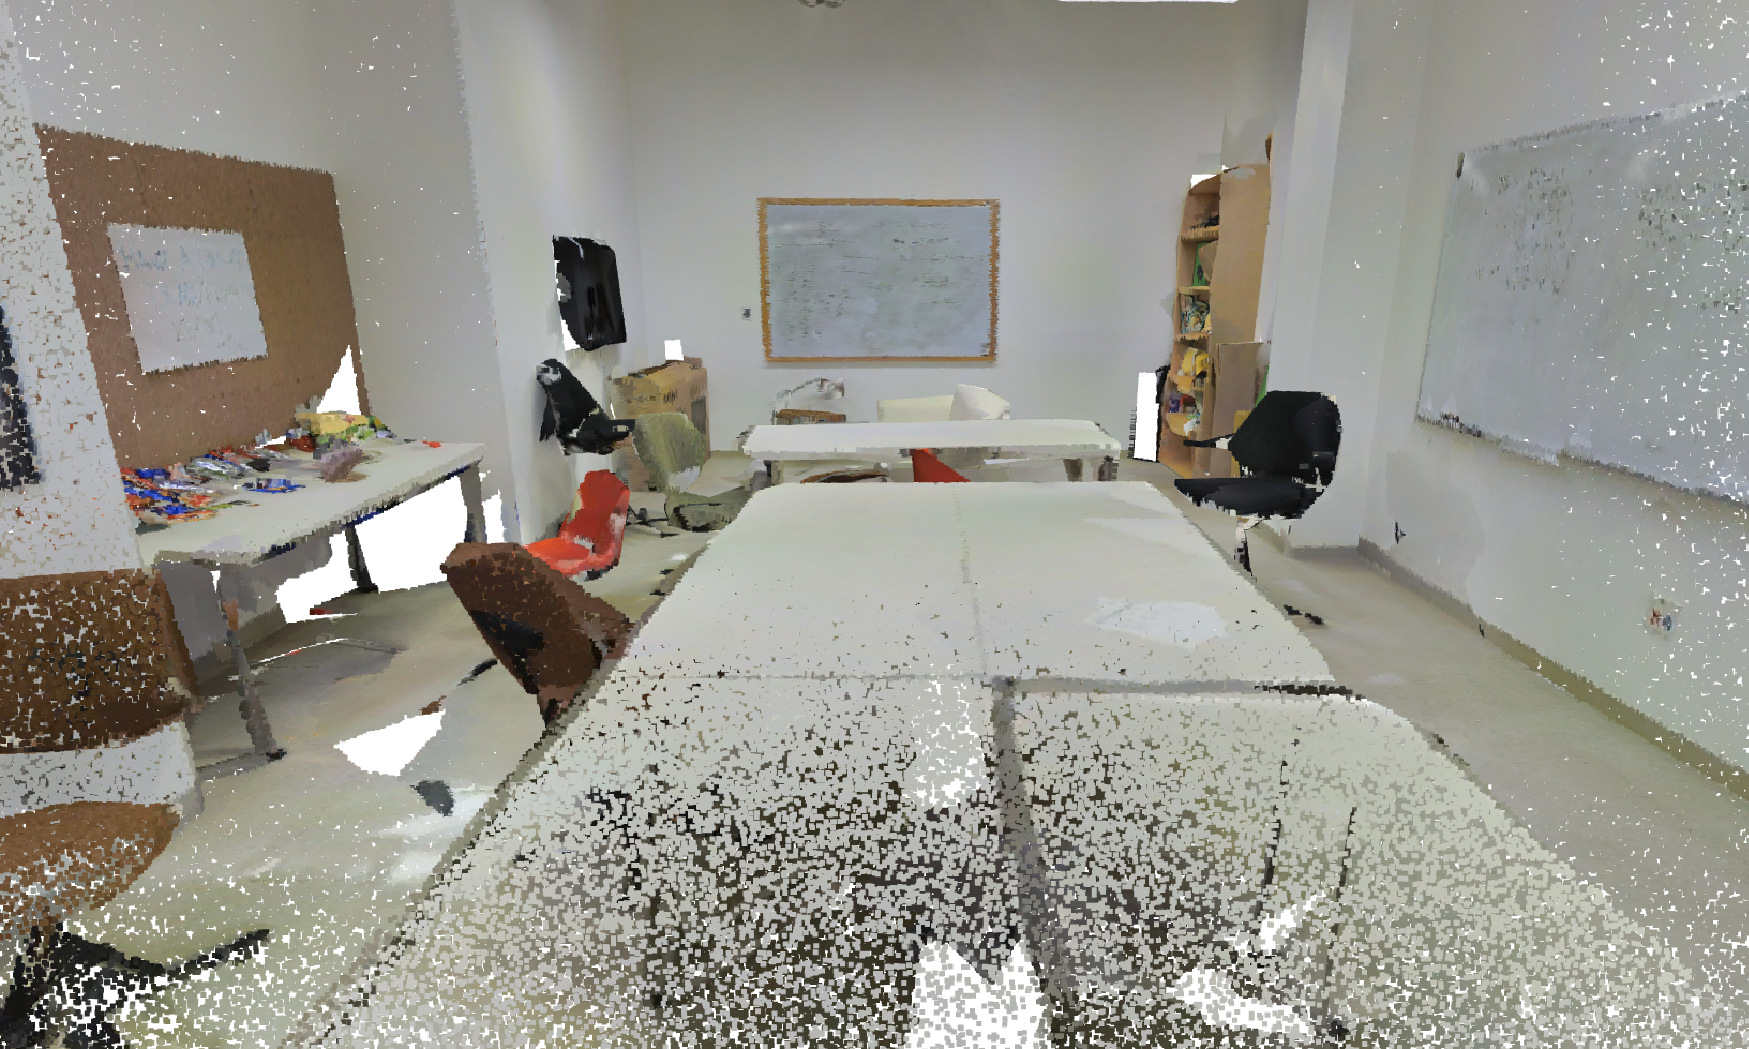
\includegraphics[width=0.35\textwidth, height=0.15\textheight]{images/seg_output/s3dis_DE/S3DIS_7_RGB.pdf} \\

        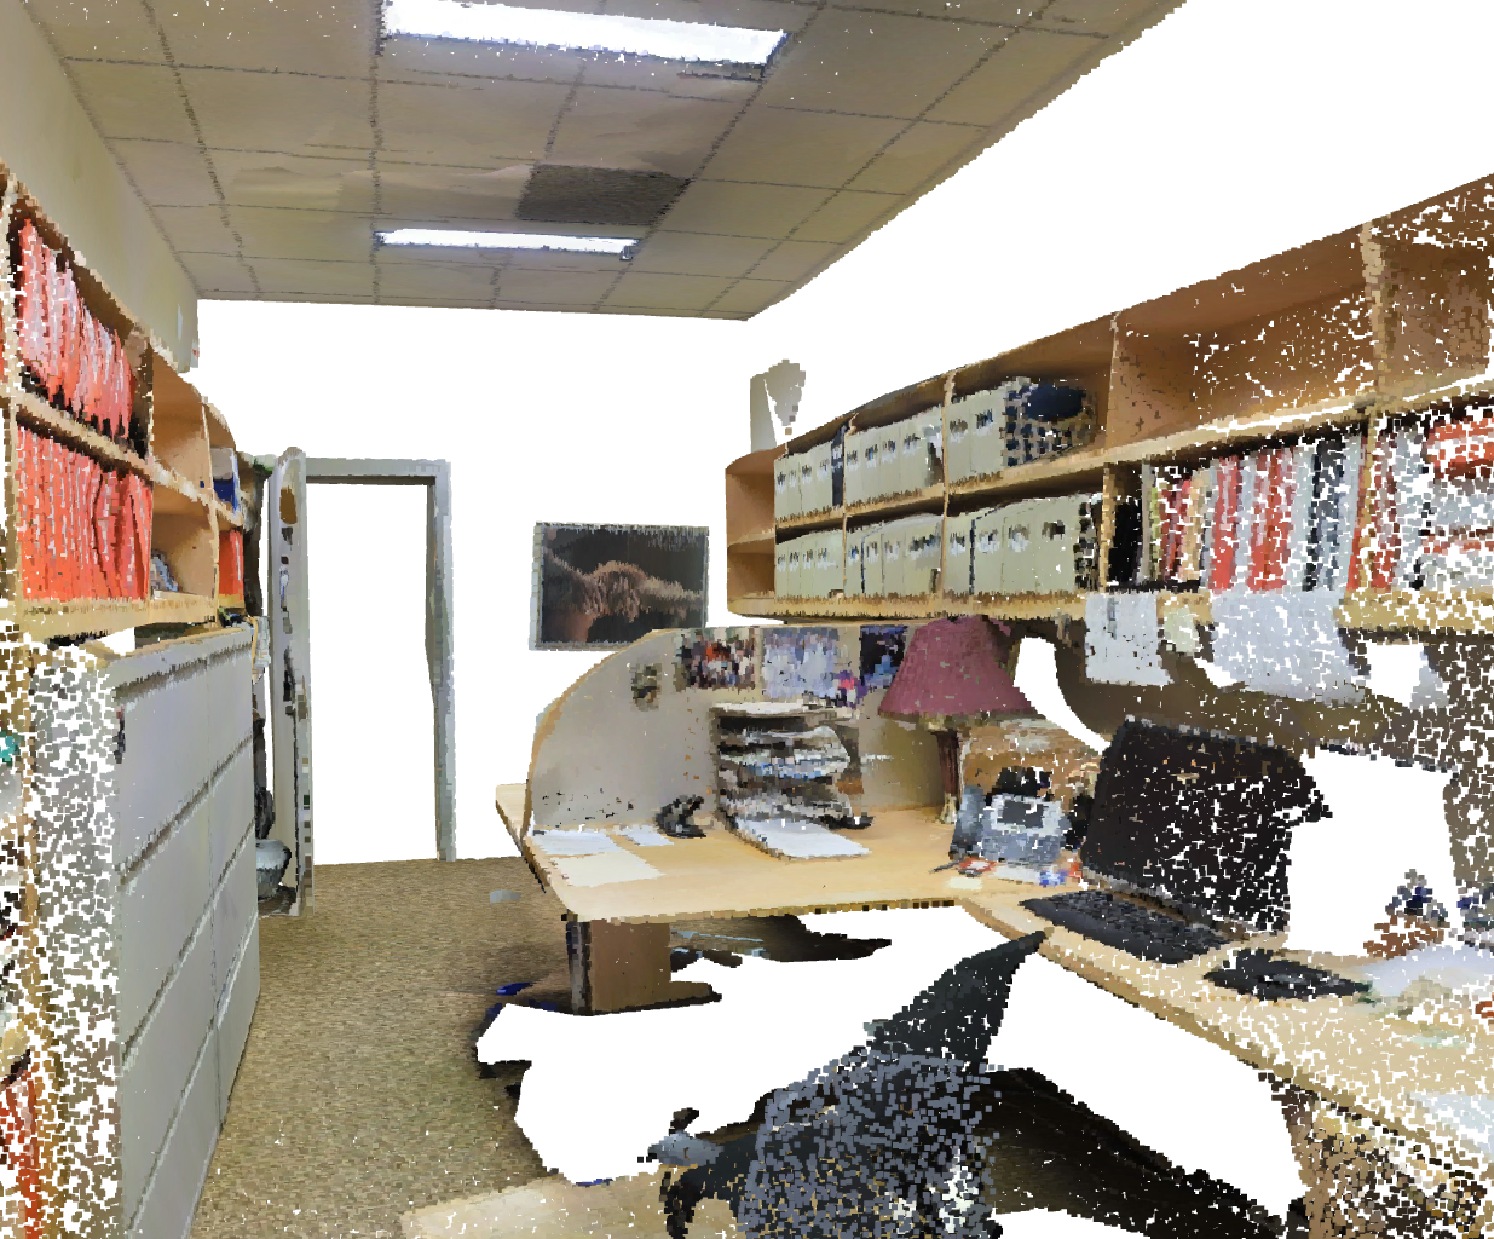
\includegraphics[width=0.35\textwidth, height=0.15\textheight]{images/seg_output/s3dis_DE/S3DIS_4_RGB.pdf} &
        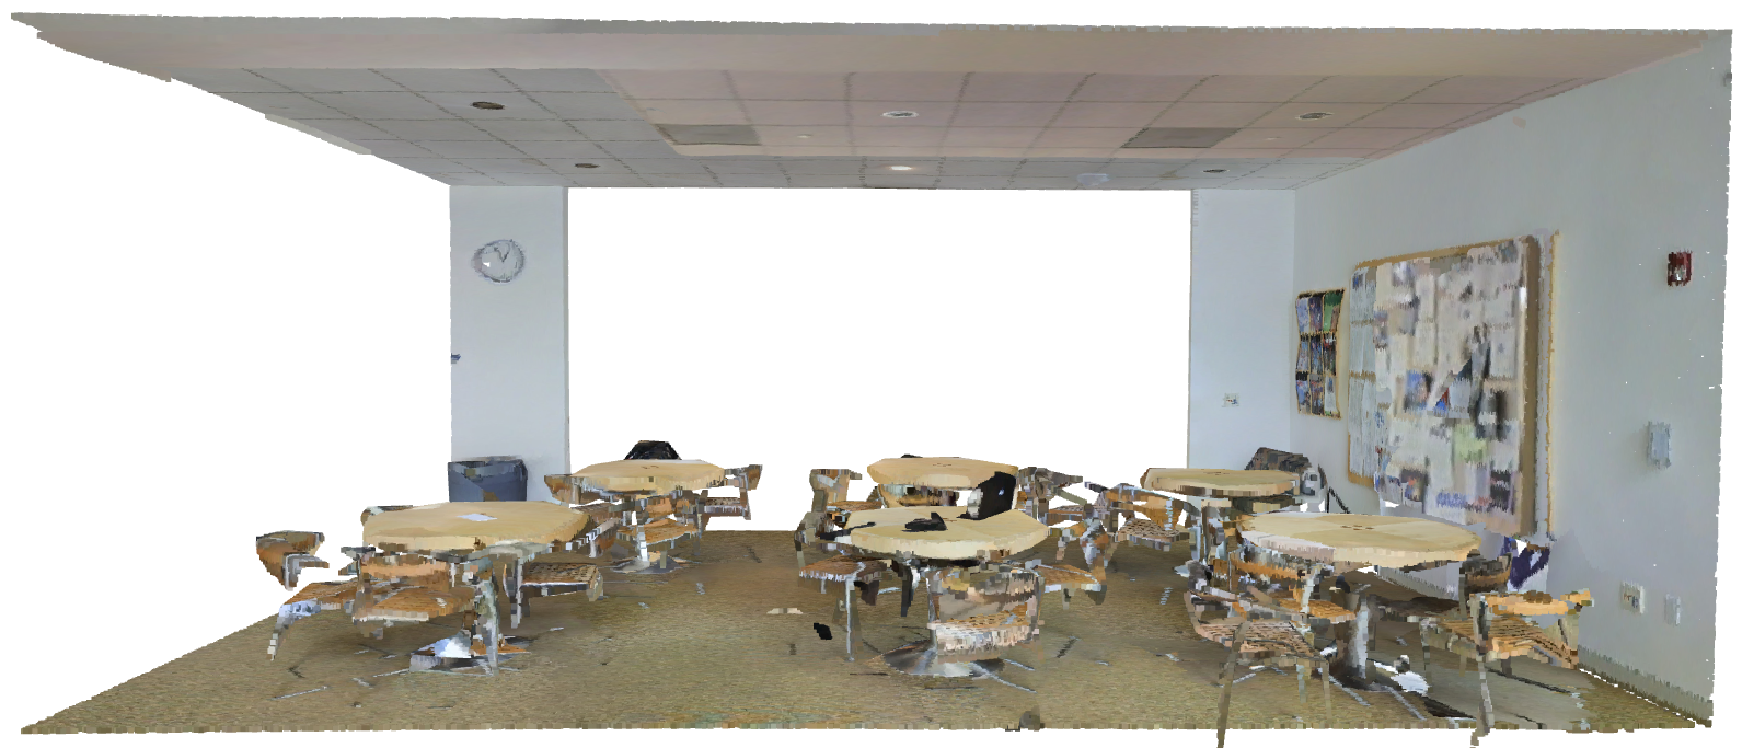
\includegraphics[width=0.35\textwidth, height=0.15\textheight]{images/seg_output/s3dis_DE/S3DIS_8_RGB.pdf} \\
    \end{tabular}
    \caption{Illustration of the point cloud with various rooms in a building from the S3DIS dataset.}
    \label{fig:s3dis_get_vis}
\end{figure}

\begin{figure}
    \centering
    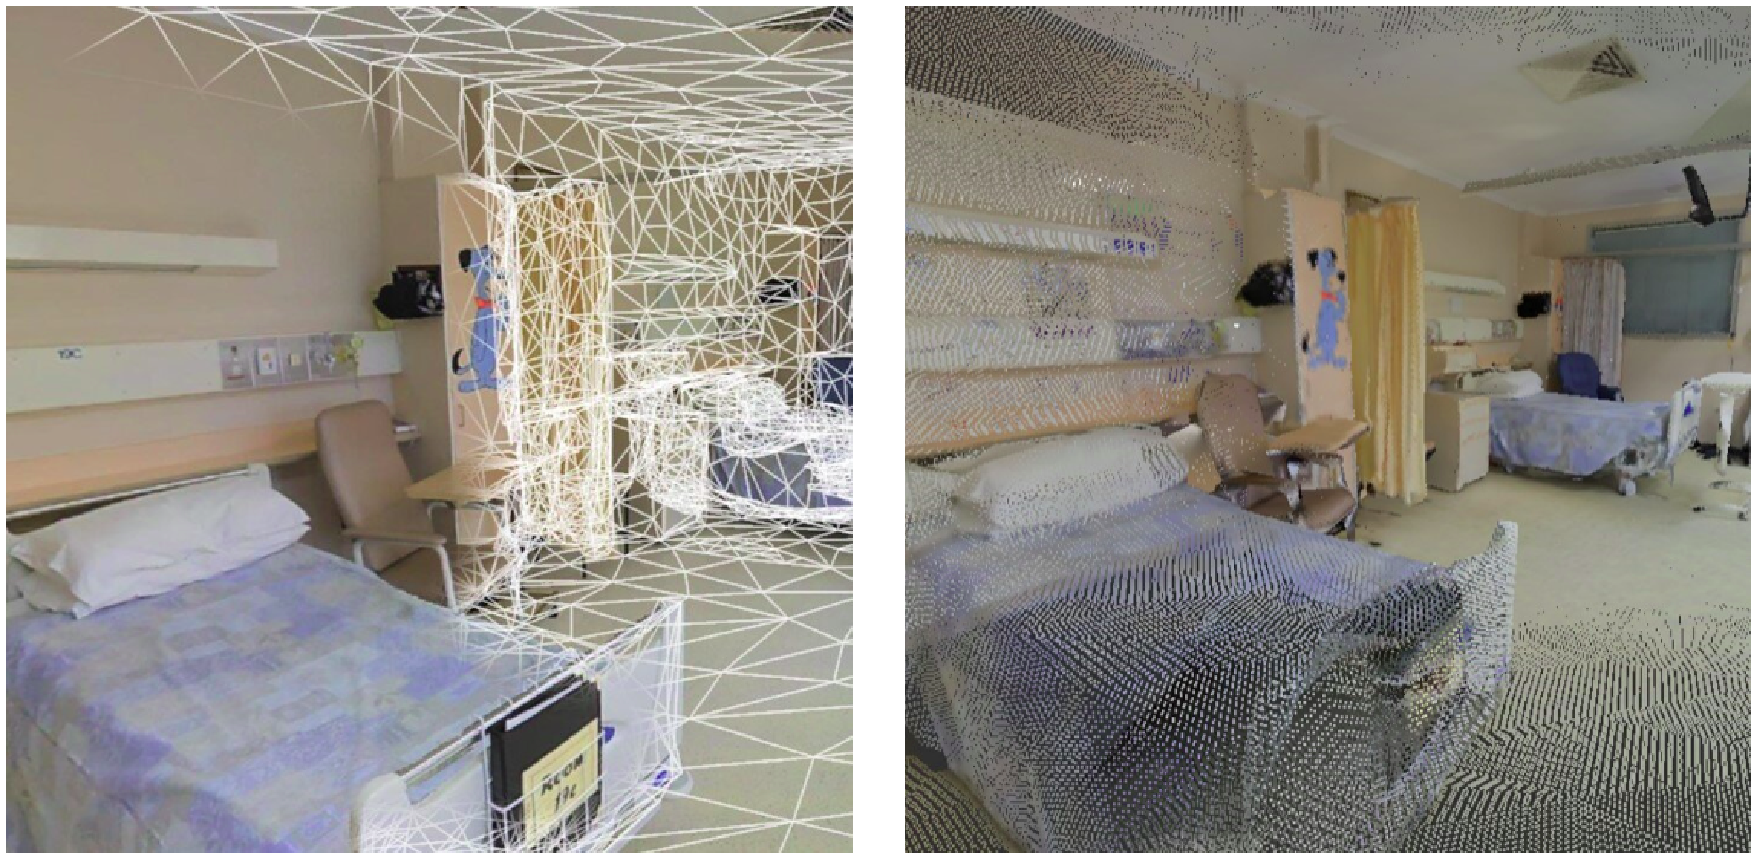
\includegraphics[scale=0.35]{images/seg_output/s3dis_DE/matterport_scan.pdf}
    \caption{Image (a) representing the triangular meshes generated from the Matterport camera and (b) depicts extracted point cloud from these traingular meshes. Image taken from \cite{matterport_scan_generation}.}
    \label{fig:how_matterport_works}
\end{figure}
\section{OOD Benchmarking}
In this section, we discuss benchmarked datasets and argue why they are chosen as benchmarking datasets.
We provided two benchmark datasets, one being Semantic3D vs S3DIS and Semantic3D vs Semantic3D (without colour).

\subsection{Semantic3D vs S3DIS}
We chose Semantic3D as the training (In-Distribution (ID)) dataset for the following reasons.
Semantic3D is a static dataset which means the high density of points in a scan compared to sequential datasets.
Semantic3D also has RGB colours as input features and XYZ and intensity values.
Having RGB in the dataset helps differentiate the Out-Of-Distribution (OOD) points from ID points.
Semantic3D has only eight training classes with outdoor scenes, and this helps in better understanding of each class and helps in better understanding of the predictions on the OOD dataset.
S3DIS is an indoor dataset with scans generated in a building.
This difference in scenes (outdoor vs indoor) makes it an ideal dataset benchmark to study.
We expect the Semantic3D trained model to detect OOD (S3DIS) dataset with relative ease and high confidence because of the enormous difference in features in the scene.

\subsection{Semantic3D vs Semantic3D (without color)}
Since our main hypothesis is that RGB colours play a significant role in detecting the OOD objects.
So we removed the colours of the Semantic3D dataset, and since the model requires RGB values for prediction, we changed the colour of points to black.w
\end{document}